% Chapter 11

\chapter{Final charged hadrons multiplicities} % Chapter title

\label{ch:mult} % For referencing the chapter elsewhere, use \autoref{ch:name}

%----------------------------------------------------------------------------------------

This chapter is divided in two parts : one is focused on the discussion on the systematic uncertainties, the other presents the final multiplicities of unidentified charged hadrons, charged pions, charged kaons and protons/antiprotons extracted from SIDIS of 160 GeV muons off a pure proton target ($lH_2$). These results are obtained from the raw multiplicities of Chapter. \ref{ch:raw} and the correction factors of Chapter. \ref{ch:CF}.

%----------------------------------------------------------------------------------------

\section{Summary of systematic studies}

The various systematic studies that were performed are summarized hereafter.

%----------------------------------------------------------------------------------------

\subsection{Systematic uncertainty associated to the RICH unfolding}

The first stage of pion identification is based on the likelihood ratios : $LH(\pi)/LH(2^{nd})$ and $LH(\pi)/LH(bg)$. These cuts are optimized to minimize the
pions misidentified as kaons. The systematic error associated to the selection of these cuts is performed varying the cuts around optimized values. Two sets of
cuts \textit{loose} and \textit{severe} were used (see Table \ref{tab:loose.severe})

\begin{table}[!h]
	\centering
	\begin{tabular}{ccccccc}
		\hline
		 & \multicolumn{3}{c}{Loose} & \multicolumn{3}{c}{Severe} \\
		\hline
		 & $\pi$ & $K$ & $p(\bar{p})$ & $\pi$ & $K$ & $p(\bar{p})$ \\
		\hline
		$\frac{LH(\pi)}{LH(2^{nd})}$ & $> 1.00$ & $-$ & $-$ & $>1.06$ & $-$ & $-$ \\
		$\frac{LH(\pi)}{LH(bg)}$ & $> 2.00$ & $-$ & $<2.3$ $(2.2)$ & $>2.04$ & $-$ & $<2.0$ $(1.9)$ \\
		$\frac{LH(K)}{LH(2^{nd})}$ & $-$ & $>1.06$ & $-$ & $>-$ & $>1.10$ & $-$ \\
		$\frac{LH(K)}{LH(bg)}$ & $-$ & $>2.00$ & $<3.0$ $(2.9)$ & $-$ & $>2.16$ & $<2.7$ $(2.6)$ \\
		\hline
	\end{tabular}
  \caption{Set of loose and severe cuts to evaluate the RICH systematic errors.}
  \label{tab:loose.severe}
\end{table}

To evaluate the systematic error associated to the selection of the particle likelihood cuts, the particle identification is performed using the \textit{loose}
and \textit{severe} sets of likelihood cuts and the corresponding RICH probability matrices and final multiplicities are extracted ($M^{h^{\pm},loose}_{raw}$
and $M^{h^{\pm},severe}_{raw}$ respectively). The largest difference between $M^{h^{\pm},loose}_{raw}$ and $M^{h^{\pm},severe}_{raw}$ with the nominal
multiplicity $M^{h^{\pm}}_{raw}$ is taken as an estimate of the systematic error :

\begin{equation}
  \sigma^{RICH_{LH}}_{sys} = MAX(|M^{h^{\pm},loose}_{raw}-M^{h^{\pm}}_{raw}|,|M^{h^{\pm},severe}_{raw}-M^{h^{\pm}}_{raw}|)
\end{equation}

The difference between the altered RICH probability matrices and the optimal one are plotted in Figs.\ref{pic:Sysplus} and \ref{pic:Sysminus}. For pions and protons, the largest differences
($<$5\%) are observed in the high momentum $p_h$ region. For kaons the difference reaches 4\% at low $p_h$ ; small differences ($<$1\%) are observed at the
highest $p_h$ value.

A second source of systematic error is that associated with the calculation of the RICH probability matrices. This is estimated by generating two sets of altered
RICH probability matrices. As represented in Eq.\ref{eq:StatMat} the matrices are constructe using the statistical error associated to the original probability matrix elements.

\begin{figure}[!p]
	\centering
	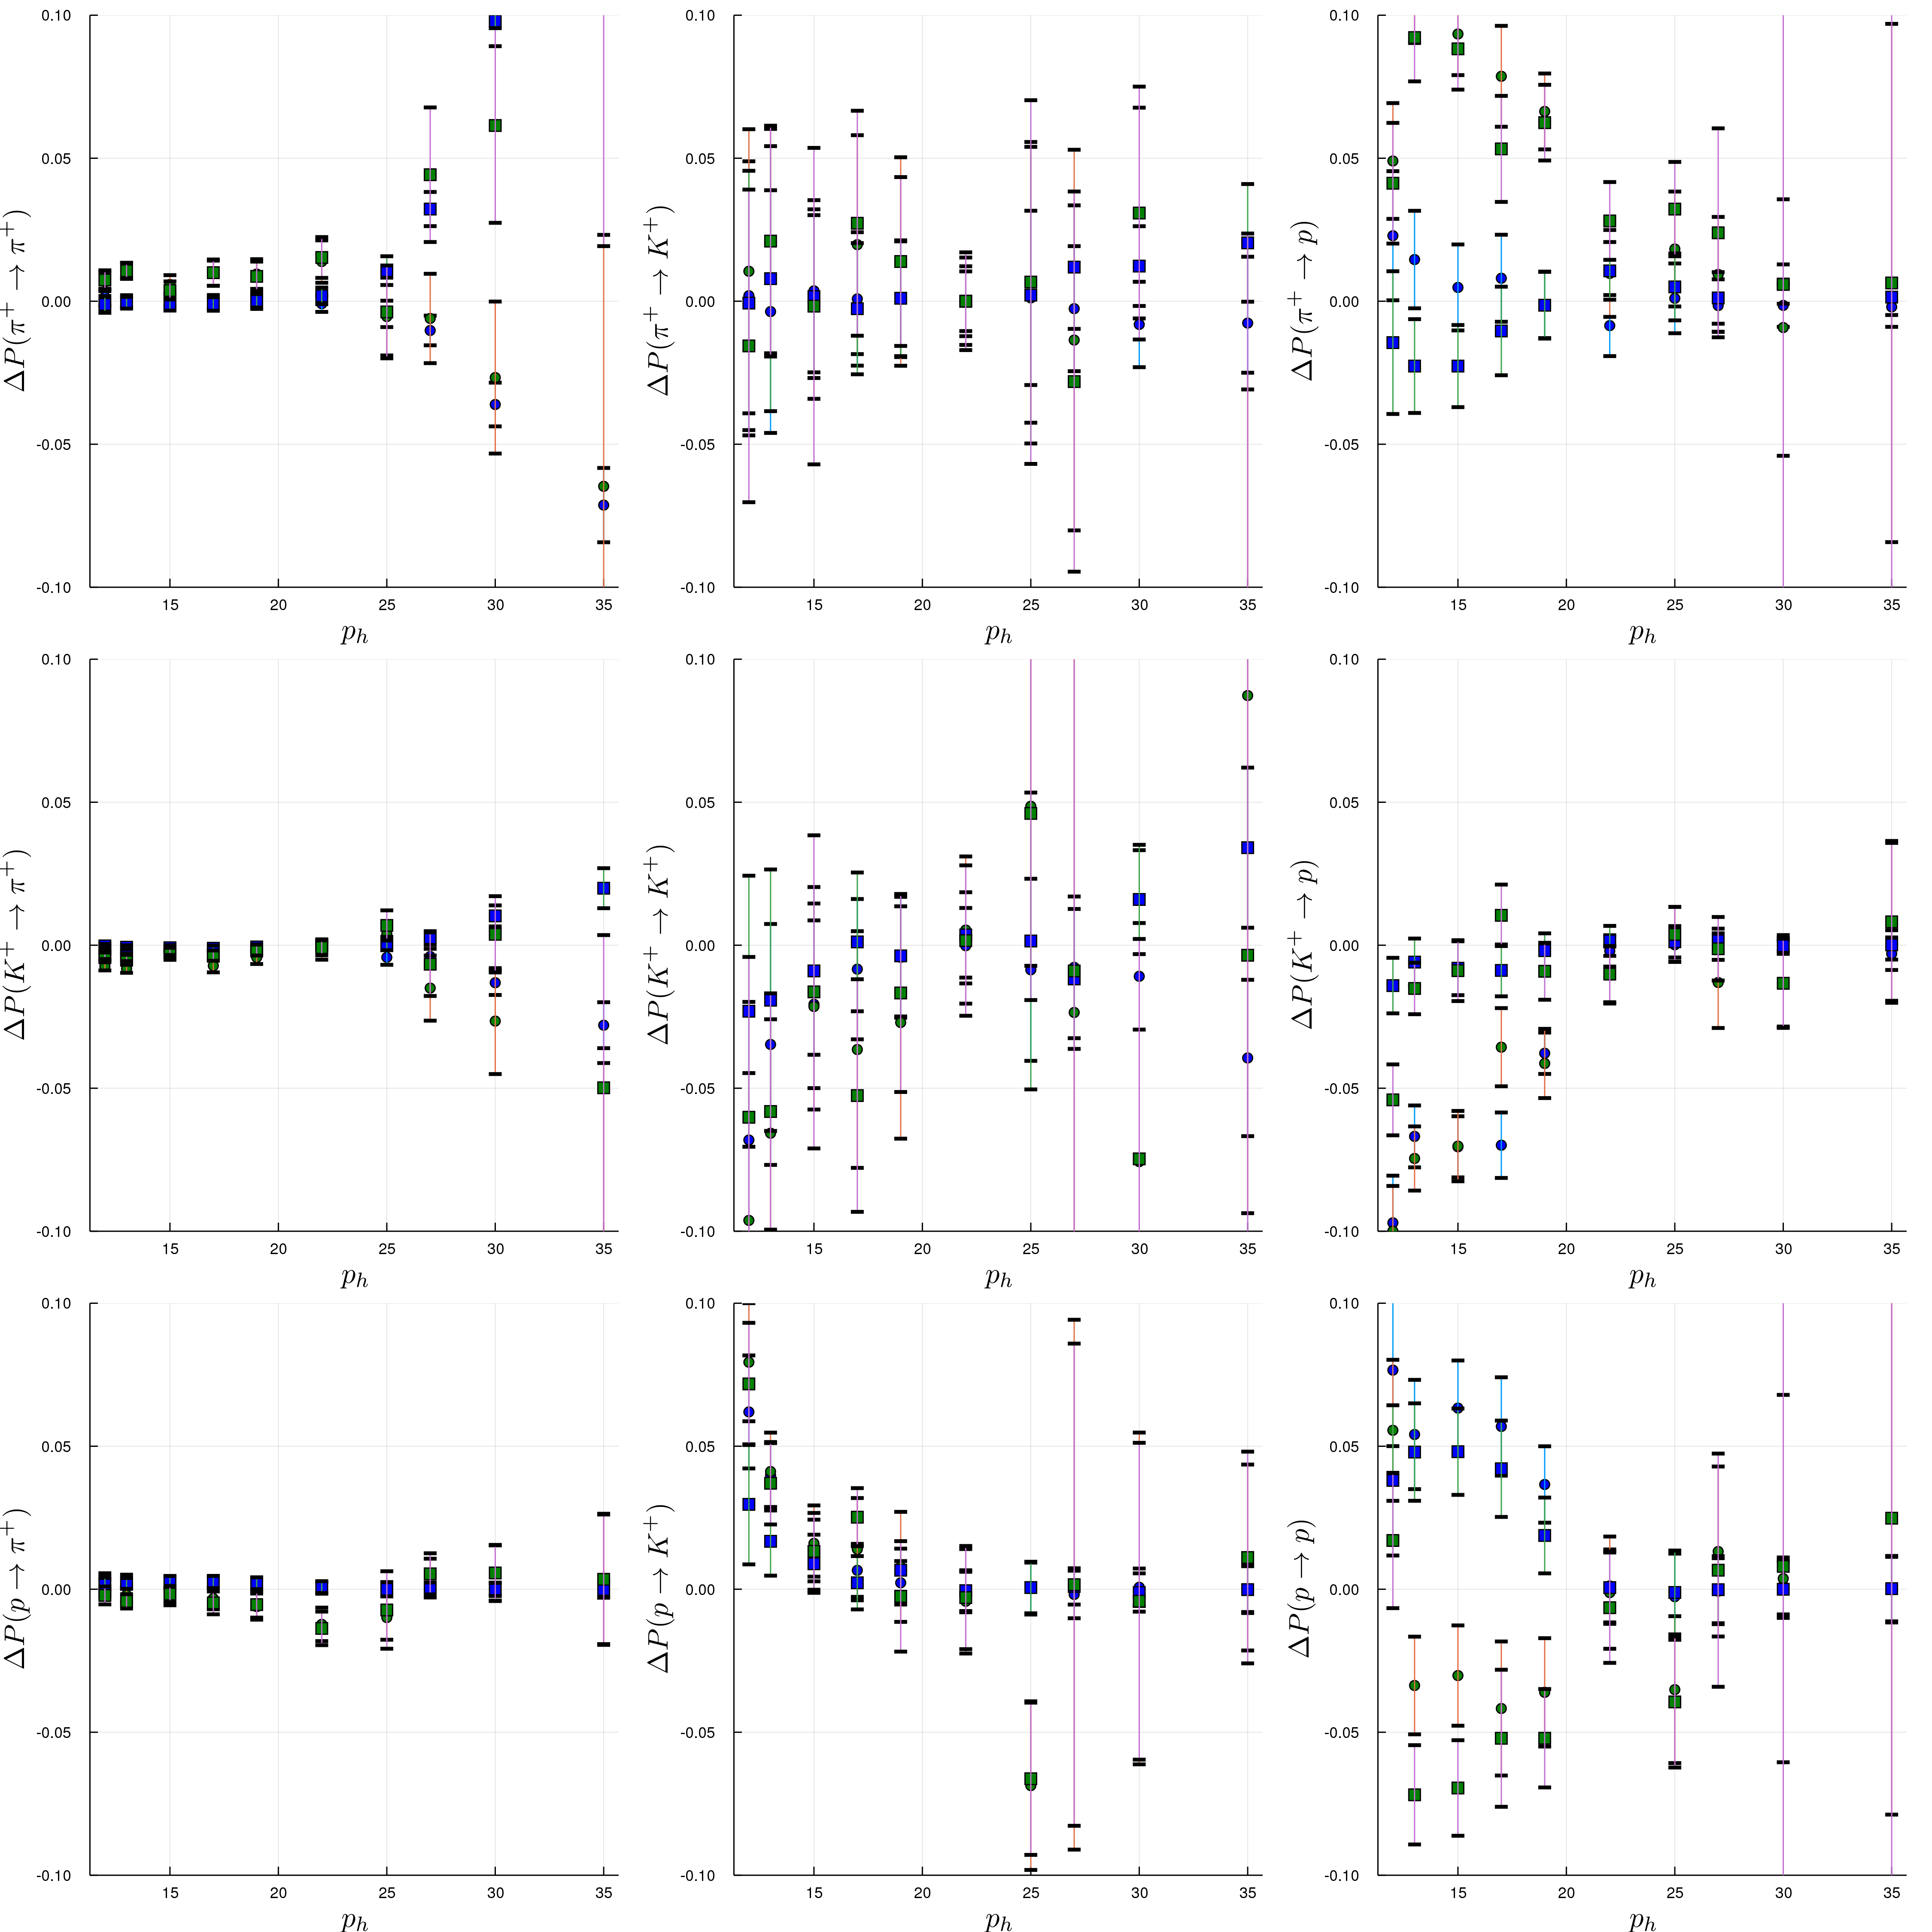
\includegraphics[scale=0.1]{./gfx/SysPlus.png}
	\caption{Difference between the identification and misidentification probabilities of loose and severe cuts with the optimal cuts for positive hadrons.}
	\label{pic:Sysplus}
\end{figure}

\begin{figure}[!p]
	\centering
	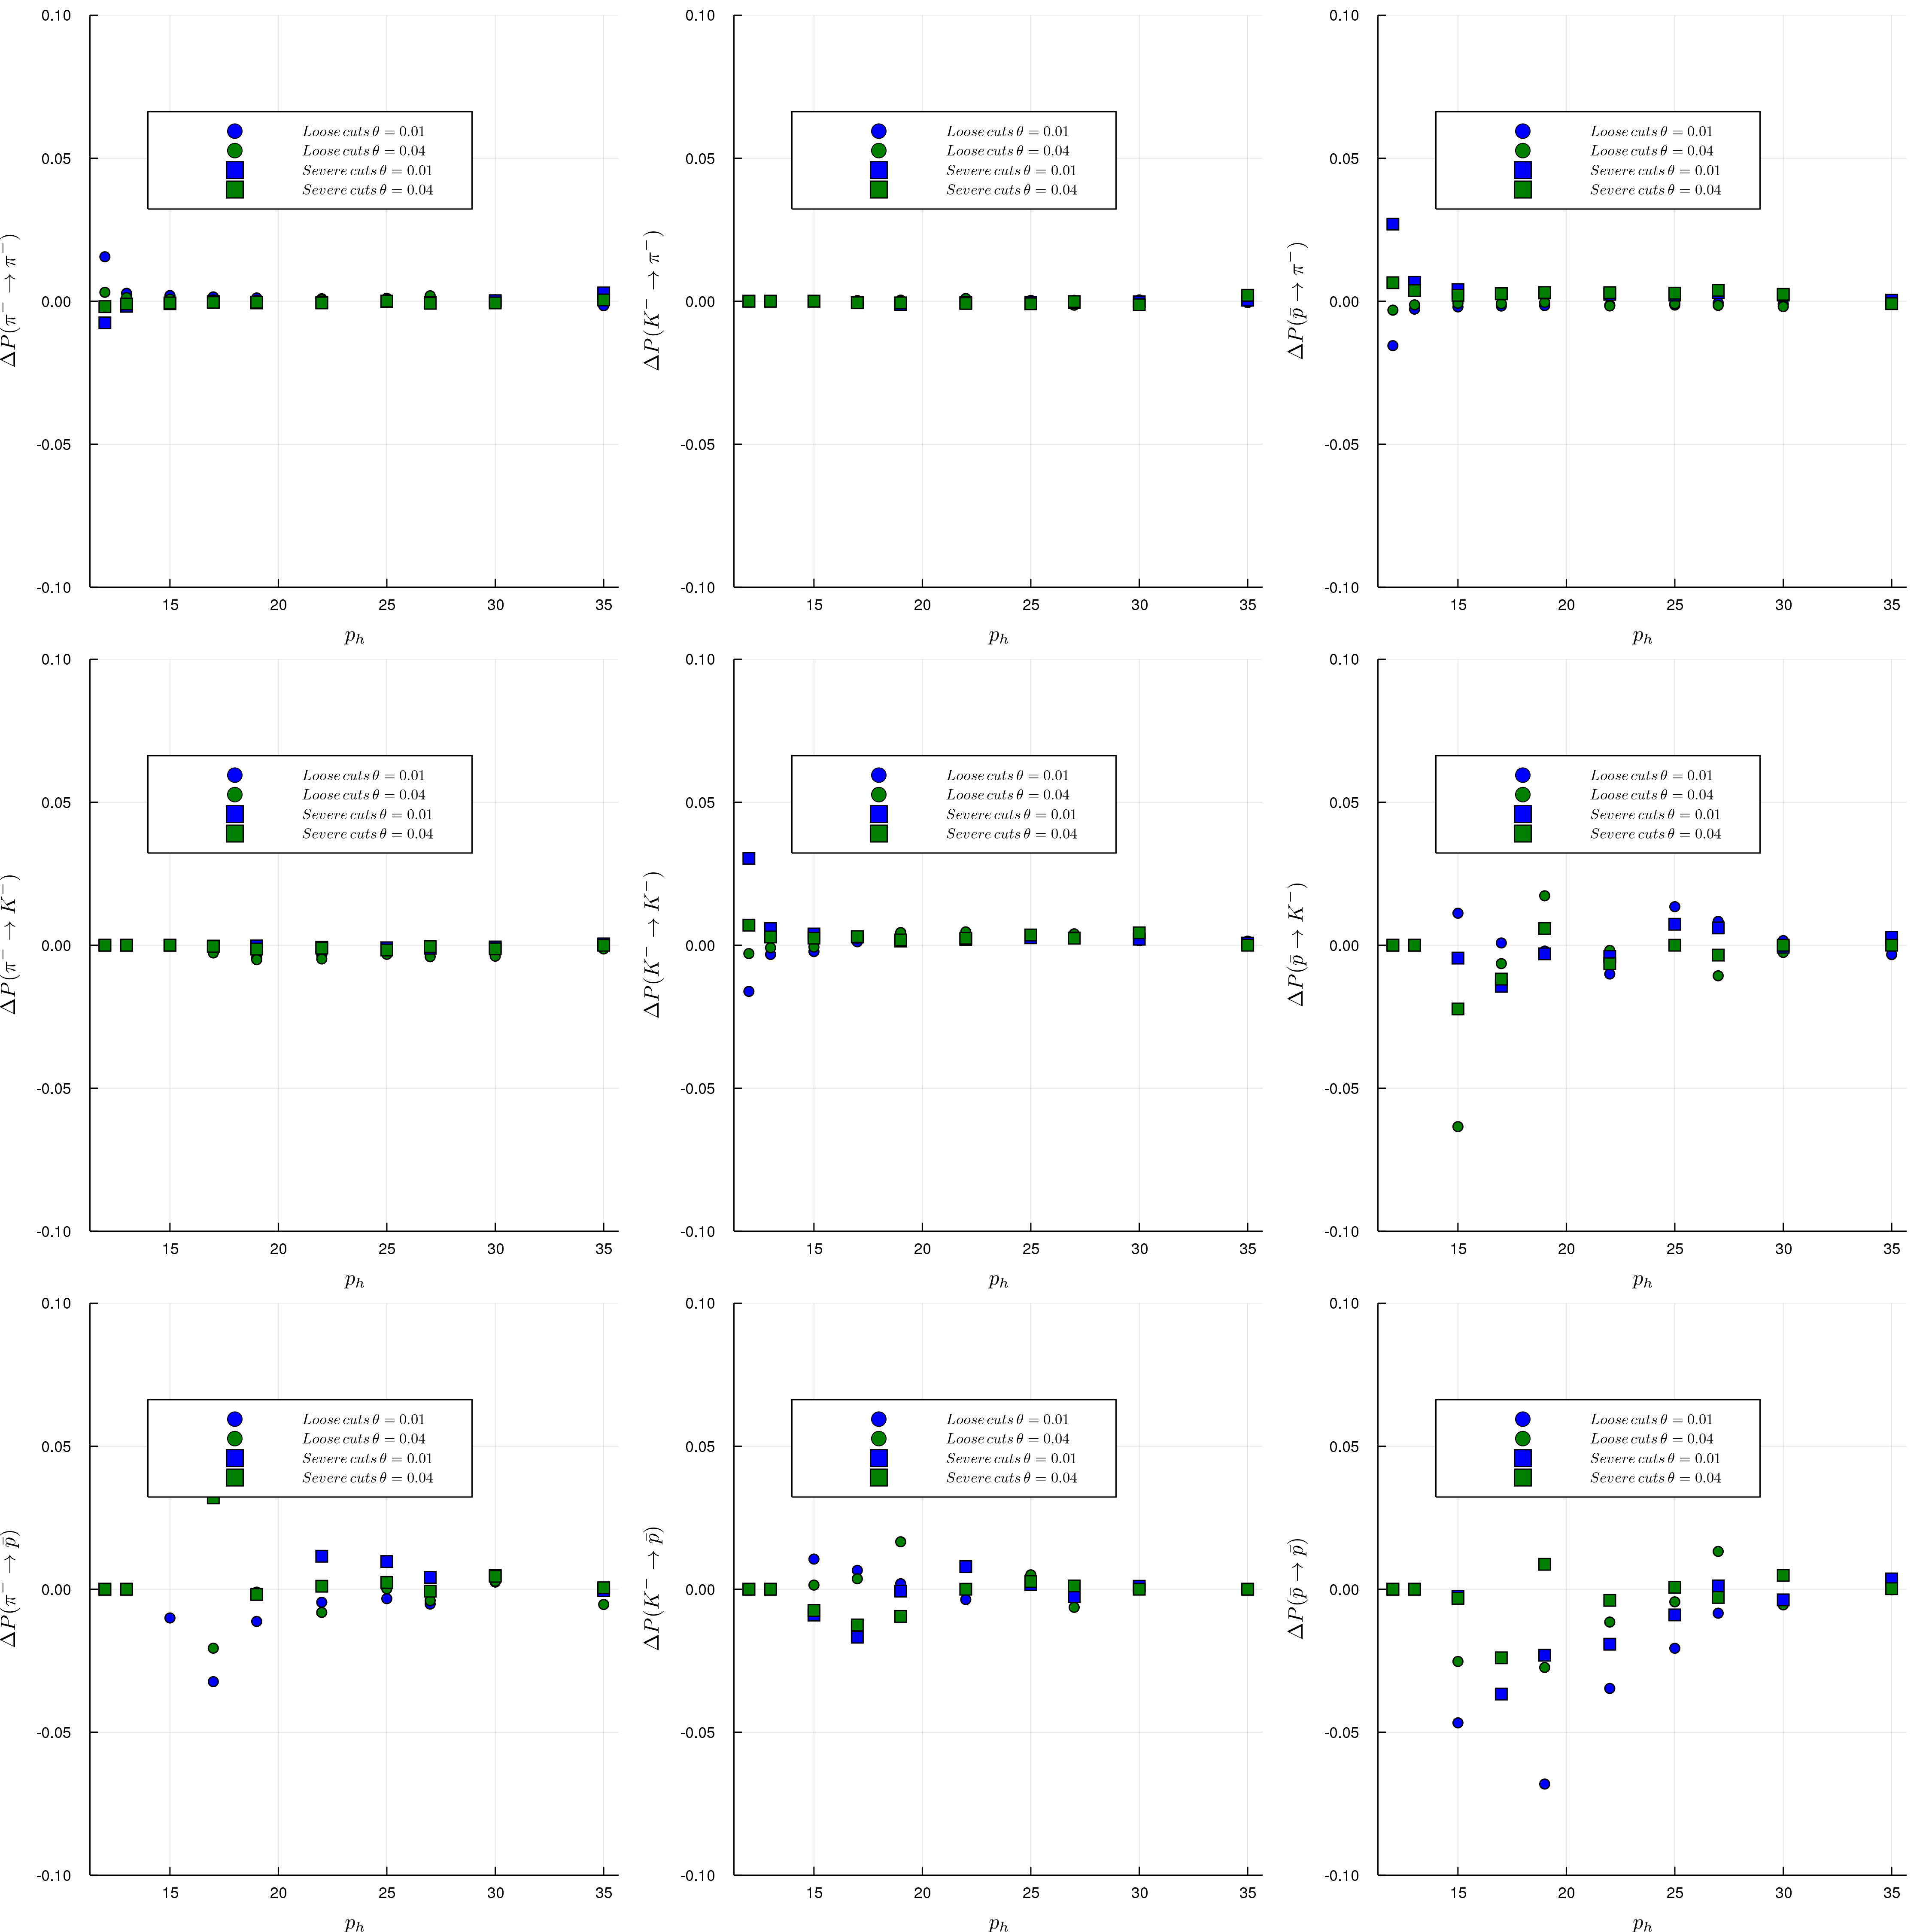
\includegraphics[scale=0.1]{./gfx/SysMinus.png}
	\caption{Difference between the identification and misidentification probabilities of loose and severe cuts with the optimal cuts for negative hadrons.}
	\label{pic:Sysminus}
\end{figure}

\begin{equation}
  M^{\pm}_{RICH}
  =
  \begin{bmatrix}
  P(\pi \rightarrow \pi)\pm\sigma_{P(\pi \rightarrow \pi)} & P(K \rightarrow \pi)\mp\sigma_{P(K \rightarrow \pi)} & P(p \rightarrow \pi)\mp\sigma_{P(p \rightarrow \pi)}\\
  P(\pi \rightarrow K)\mp\sigma_{P(\pi \rightarrow K)} & P(K \rightarrow K)\pm\sigma_{P(K \rightarrow K)} & P(p \rightarrow K)\mp\sigma_{P(p \rightarrow K)} \\
  P(\pi \rightarrow p)\mp\sigma_{P(\pi \rightarrow p)} & P(K \rightarrow p)\mp\sigma_{P(K \rightarrow p)} & P(p \rightarrow p)\pm\sigma_{P(p \rightarrow p)}
  \end{bmatrix}
	\label{eq:StatMat}
\end{equation}

The raw multiplicities $M^{h^{\pm},+}_{raw}$ and $M^{h^{\pm},-}_{raw}$ are then recalculated using the altered probability matrices. The largest difference between
$M^{h^{\pm},+}_{raw}$ and $M^{h^{\pm},-}_{raw}$ with $M^{h^{\pm}}_{raw}$ is taken as the sytematic error :

\begin{equation}
  \sigma^{RICH_{stat}}_{sys} = MAX(|M^{h^{\pm},+}_{raw}-M^{h^{\pm}}_{raw}|,|M^{h^{\pm},-}_{raw}-M^{h^{\pm}}_{raw}|)
\end{equation}

The final systematic uncertainty associated to the particle identification and unfolding correction ($\sigma^{RICH}_{sys}$) is the largest value of $\sigma^{RICH_{stat}}_{sys}$ and $\sigma^{RICH_{LH}}_{sys}$. The error goes from $<$ 0.2\% at low $y$ for all $x$ and $z$ bins to $\sim$ 20\% for high $y$ and high $z$, where multiplicities are low.

%------------------------------------------------

\subsection{Systematic uncertainty associated to the stability of data over time}

The data samples used in the analysis were recorded over a period of 5 weeks. As a quality check, the raw charged hadron multiplicities from period P07 and from the average over flux of all periods were compared. The results were found to be be compatible within statistical fluctuations for all unidentified hadrons, pions, kaons and protons (Figs. \ref{pic:hMultTime} to \ref{pic:pMultTime}). Consequently, no systematic error will be assigned for the data compatibility.

\begin{sidewaysfigure}[p]
  \centering
	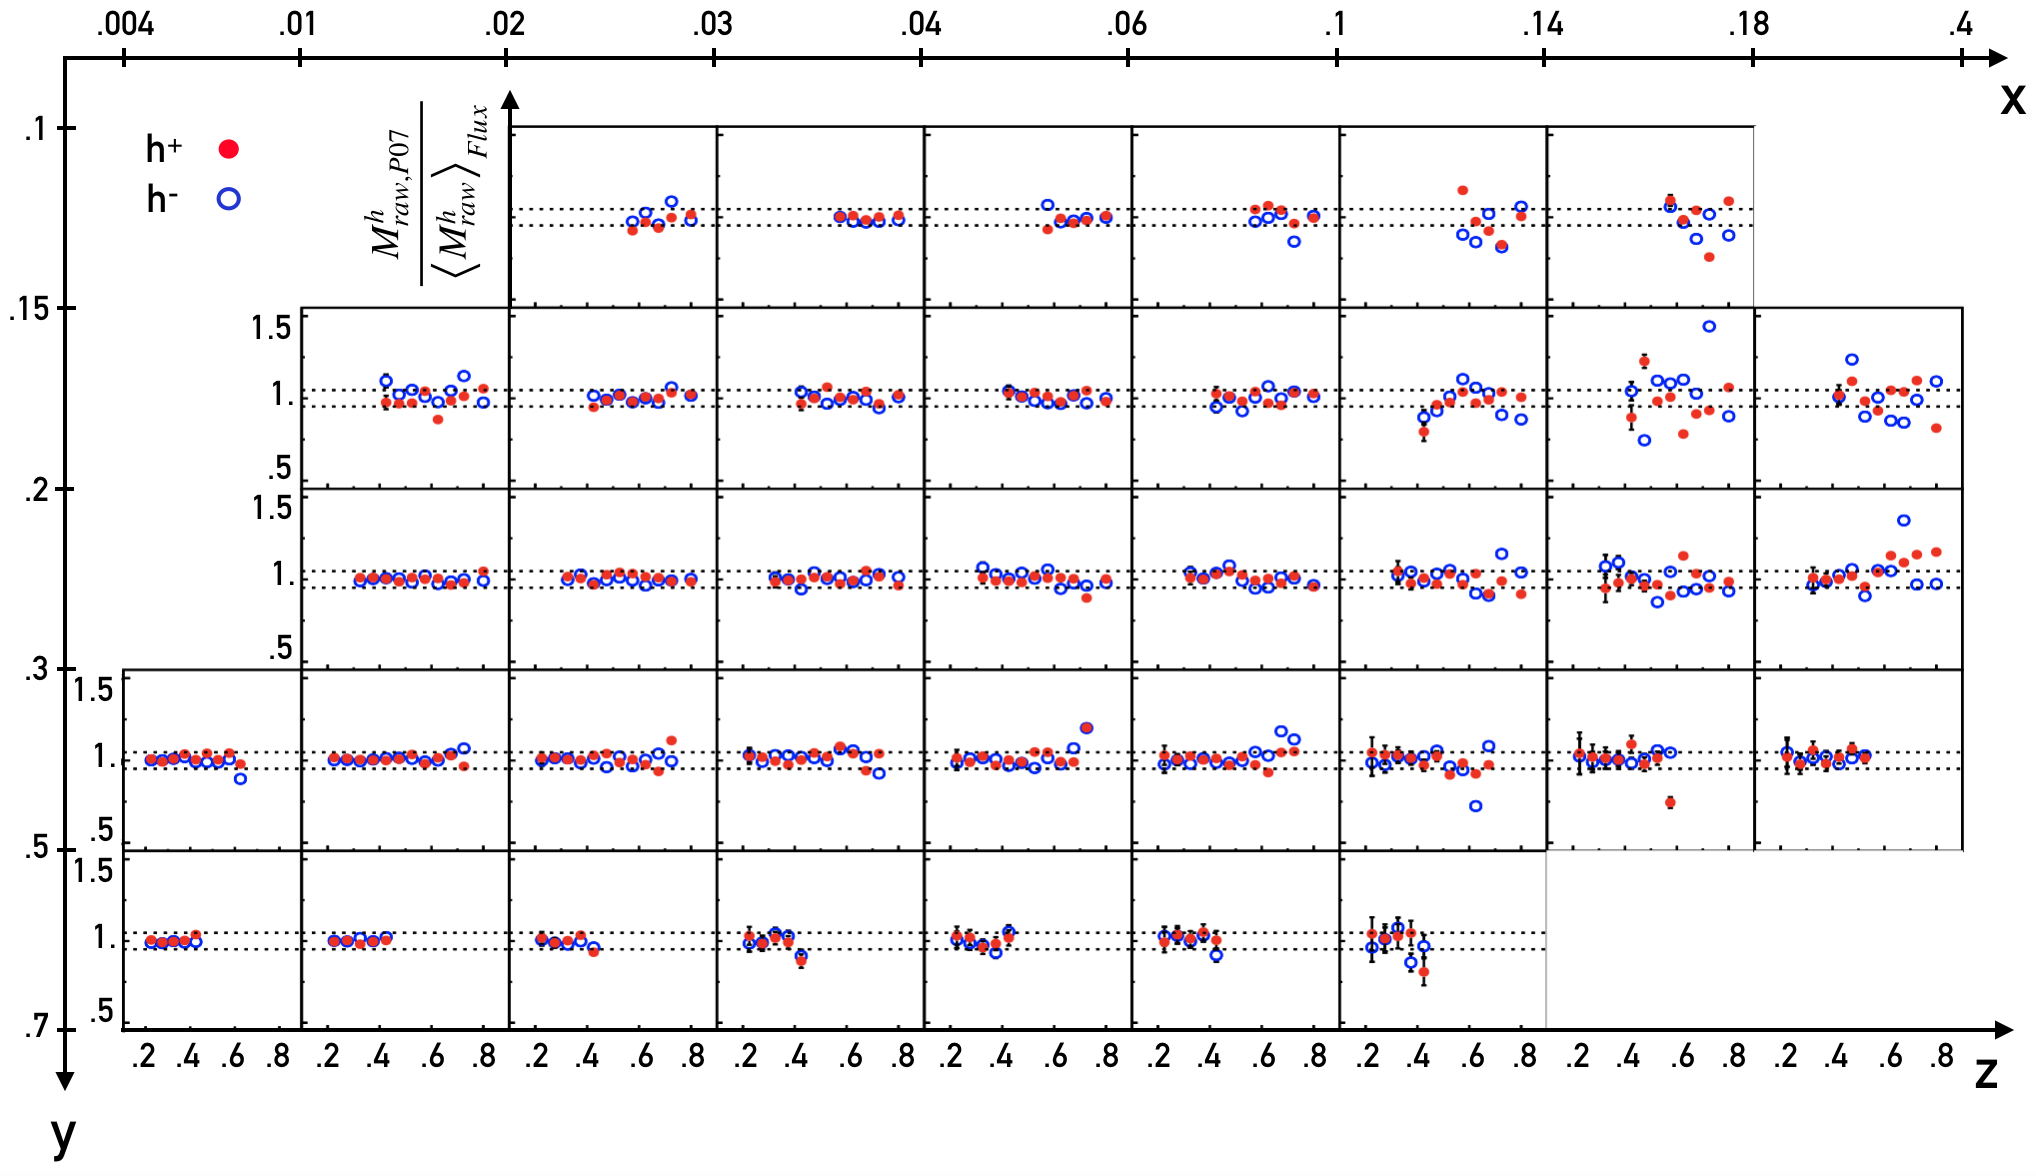
\includegraphics[scale=0.7]{./gfx/SysTimeMult.png}
	\caption{Ratio of P07 raw multiplicities over the raw multiplicities of all periods averaged over flux versus $z$. The red markers are for positive hadrons and the blue markers for negative hadrons. Each column corresponds to a given $x$ bin and each row to a given $y$ bin.}
	\label{pic:hMultTime}
\end{sidewaysfigure}

\begin{sidewaysfigure}[p]
  \centering
	% 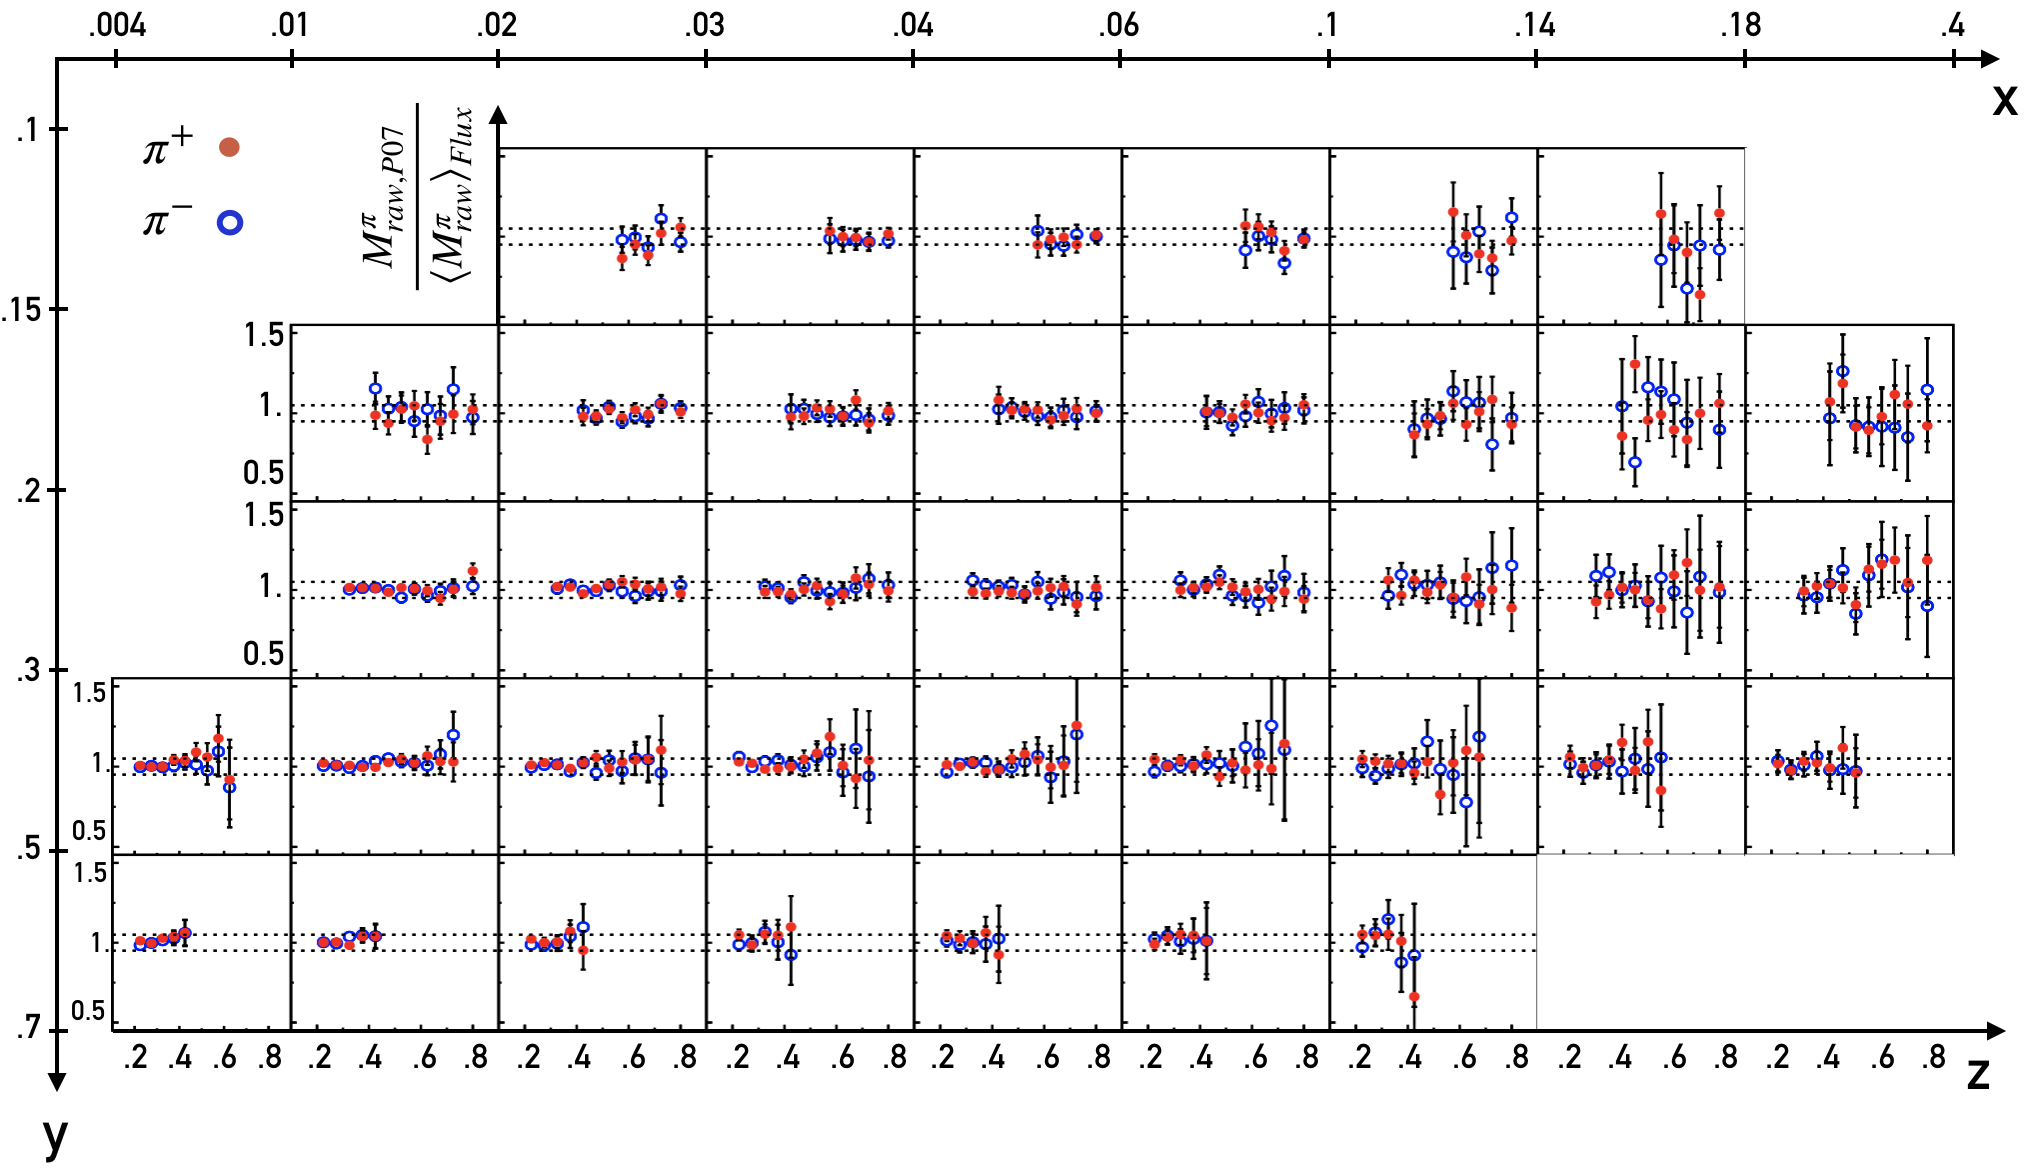
\includegraphics[scale=0.85]{./gfx/SysTimeMultpi.png}
	\caption{Same as Fig. \ref{pic:hMultTime} but for pion multiplicities.}
	\label{pic:piMultTime}
\end{sidewaysfigure}

\begin{sidewaysfigure}[p]
  \centering
	% 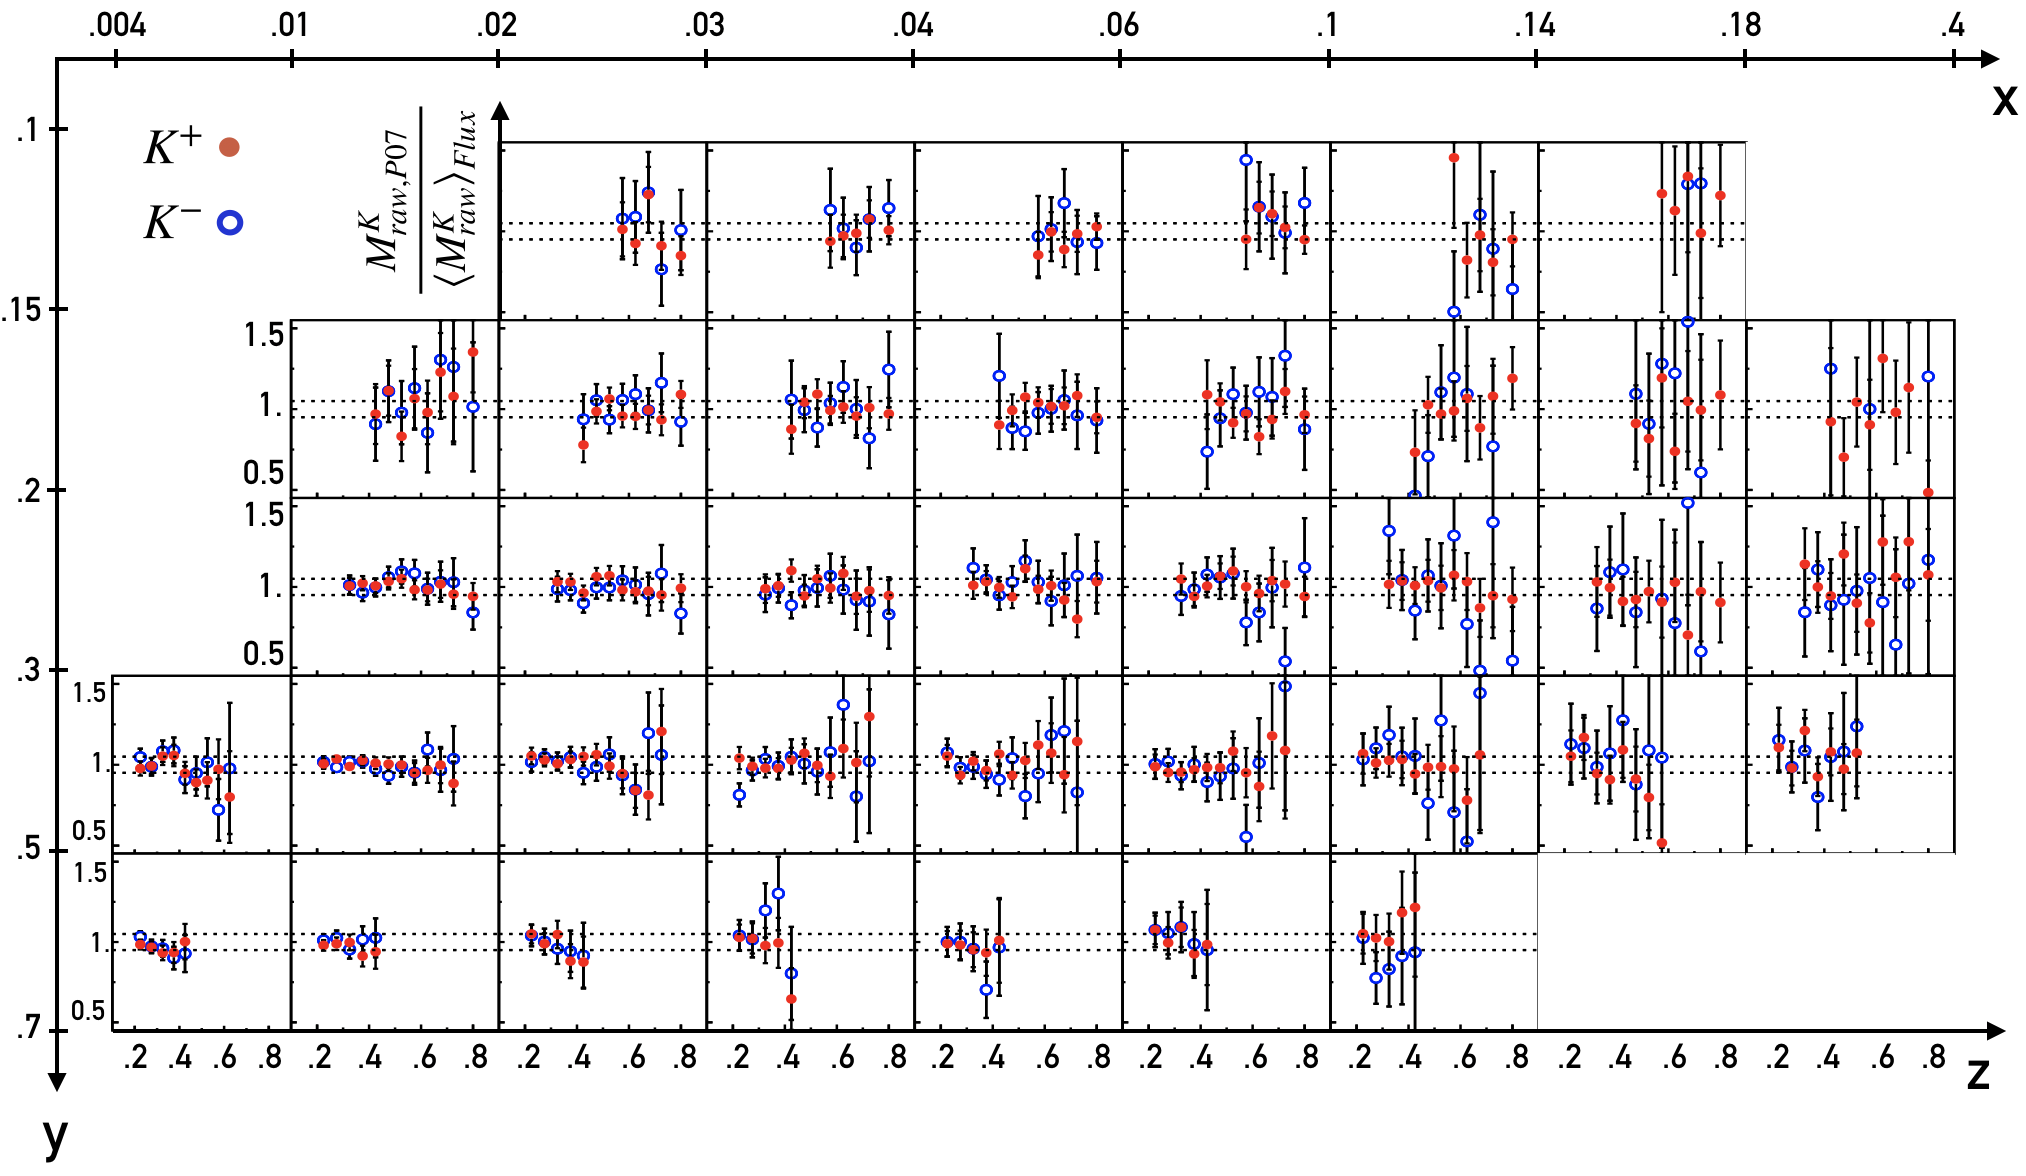
\includegraphics[scale=0.85]{./gfx/SysTimeMultk.png}
	\caption{Same as Fig. \ref{pic:hMultTime} but for kaon multiplicities.}
	\label{pic:kMultTime}
\end{sidewaysfigure}

\begin{sidewaysfigure}[p]
  \centering
	% 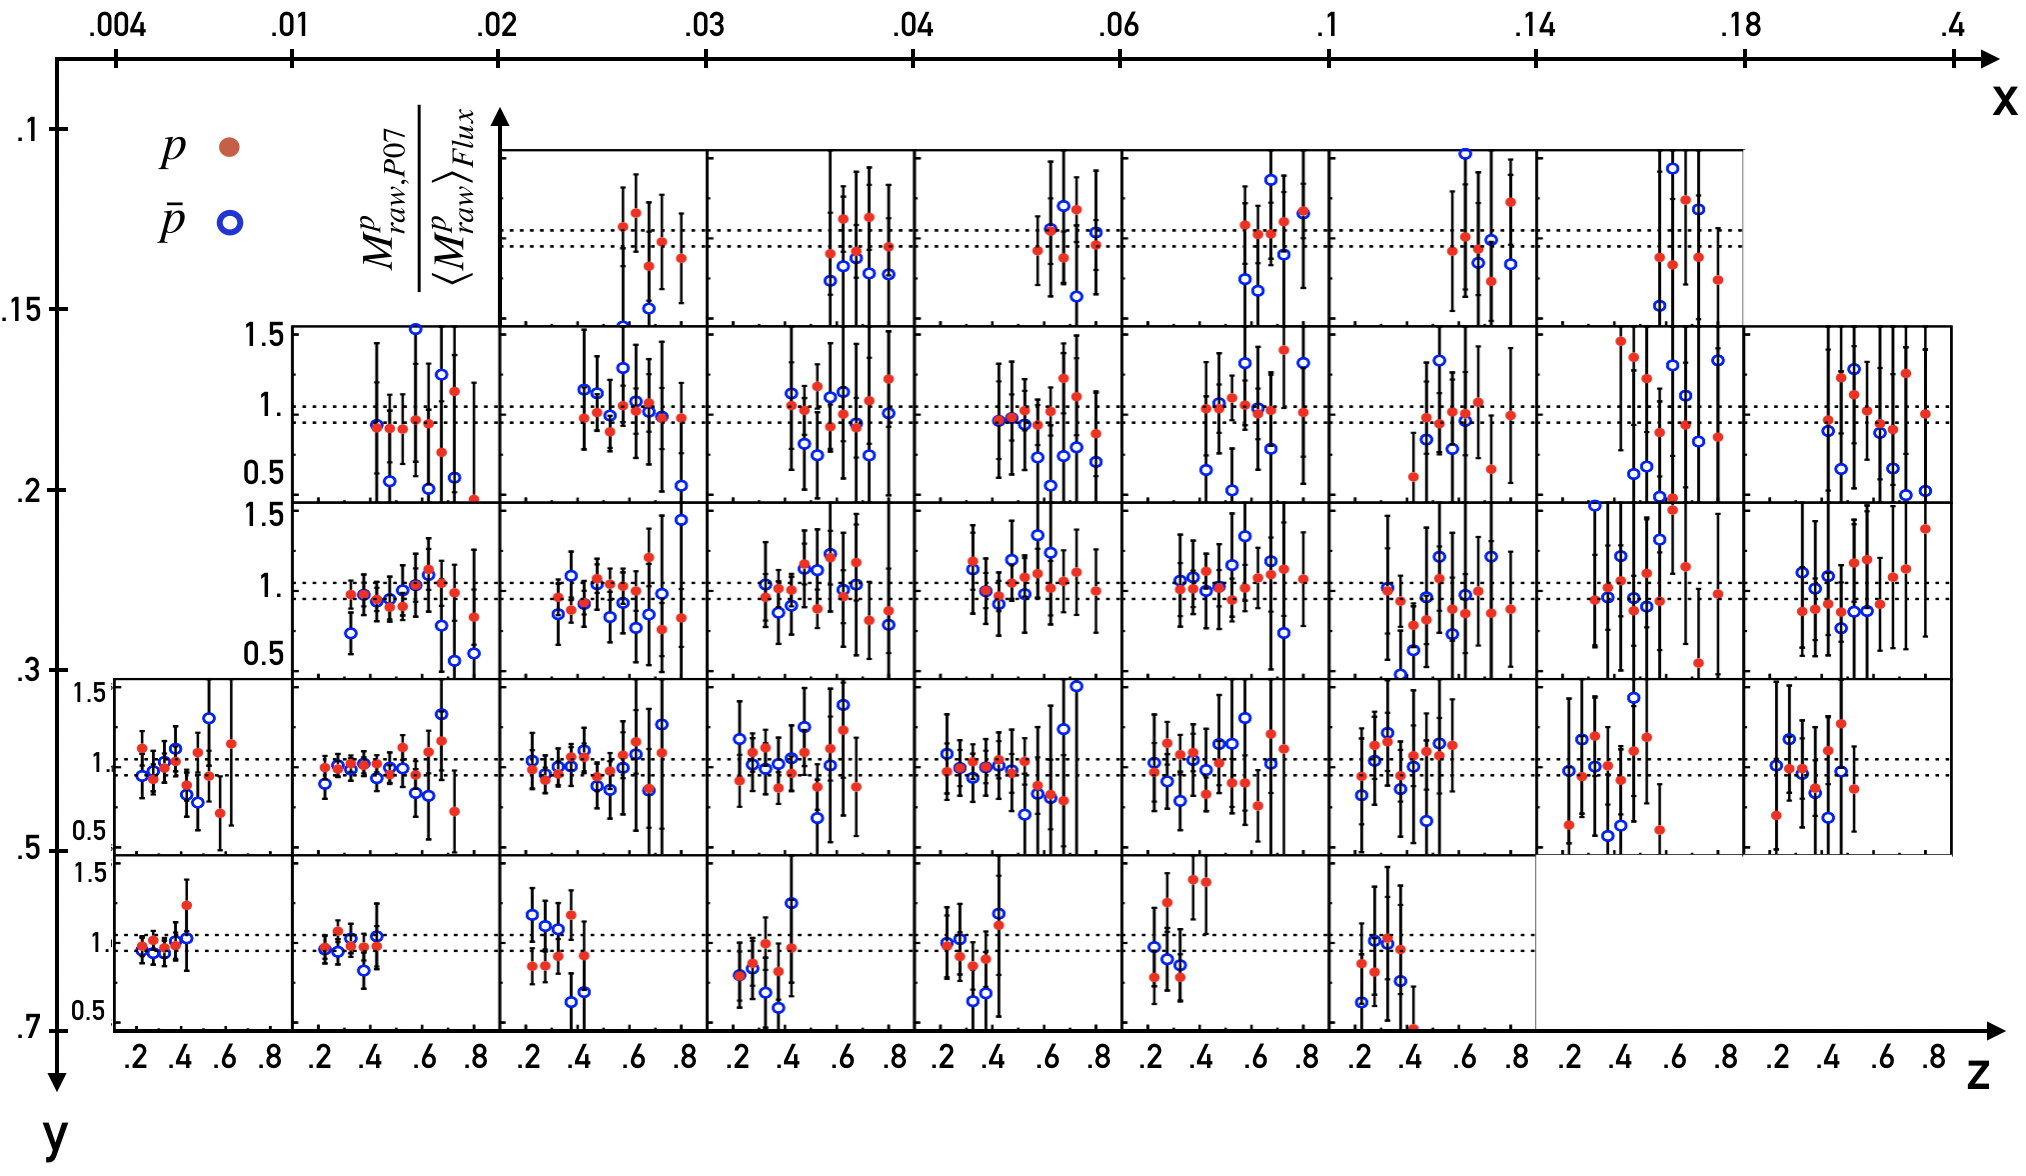
\includegraphics[scale=0.85]{./gfx/SysTimeMultp.png}
	\caption{Same as Fig. \ref{pic:hMultTime} but for proton multiplicities.}
	\label{pic:pMultTime}
\end{sidewaysfigure}

%------------------------------------------------

\subsection{Systematic uncertainty associated to the stability of data over beam charge}

The data samples used in the analysis were recorded with two different beam charges. Using the same method than in the previous subsection, a comparison was made for both beam charges and the results were compatible within statistical fluctuations. Consequently, no systematic error will be assigned for the beam charge change.

%------------------------------------------------

\subsection{Systematic uncertainty associated to Monte Carlo sample : DJANGOH dependence}

To determine the acceptance dependence with the physical model chosen, different PDF sets were used to generate different MC samples. Moreover different JETSET parameters were also used \cite{PDFsys}. For each sample the acceptance is calculated and the hadron multiplicities are corrected with each acceptance. The systematic uncertainty on the acceptance, considering two acceptances $A^h$ and $A'^h$, is estimed in each kinematic bin ($x$,$y$,$z$) :

\begin{equation}
  \sigma^{A^h}_{syst} \leq \frac{\frac{A'^h}{A^h}-1}{2}M^h_{corr_acc}
\end{equation}

The value of $\sigma^{A^h}_{syst}$ was found to be of $\sim$ 5\%.

Another error concerns the z-vertex dependence : the target can be separated into 4 different parts and the sum of multiplicities extracted from each part is then compared (Fig. \ref{pic:Zvertexsum}). From this comparison, a conservative systematic error of $\sim$ 5\% was derived.

\begin{figure}[!h]
  \centering
	\subfloat[]{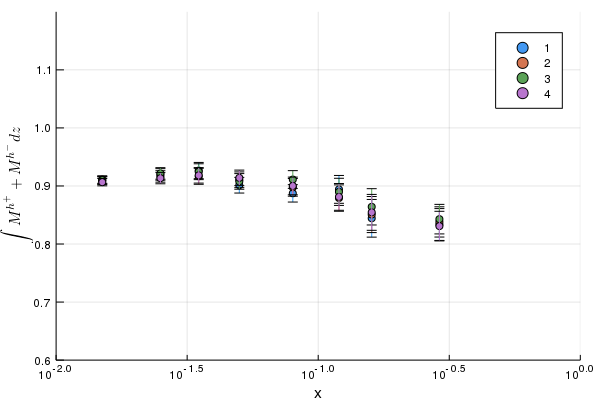
\includegraphics[scale=0.5]{./gfx/SumVertex.png}} \\
  \subfloat[]{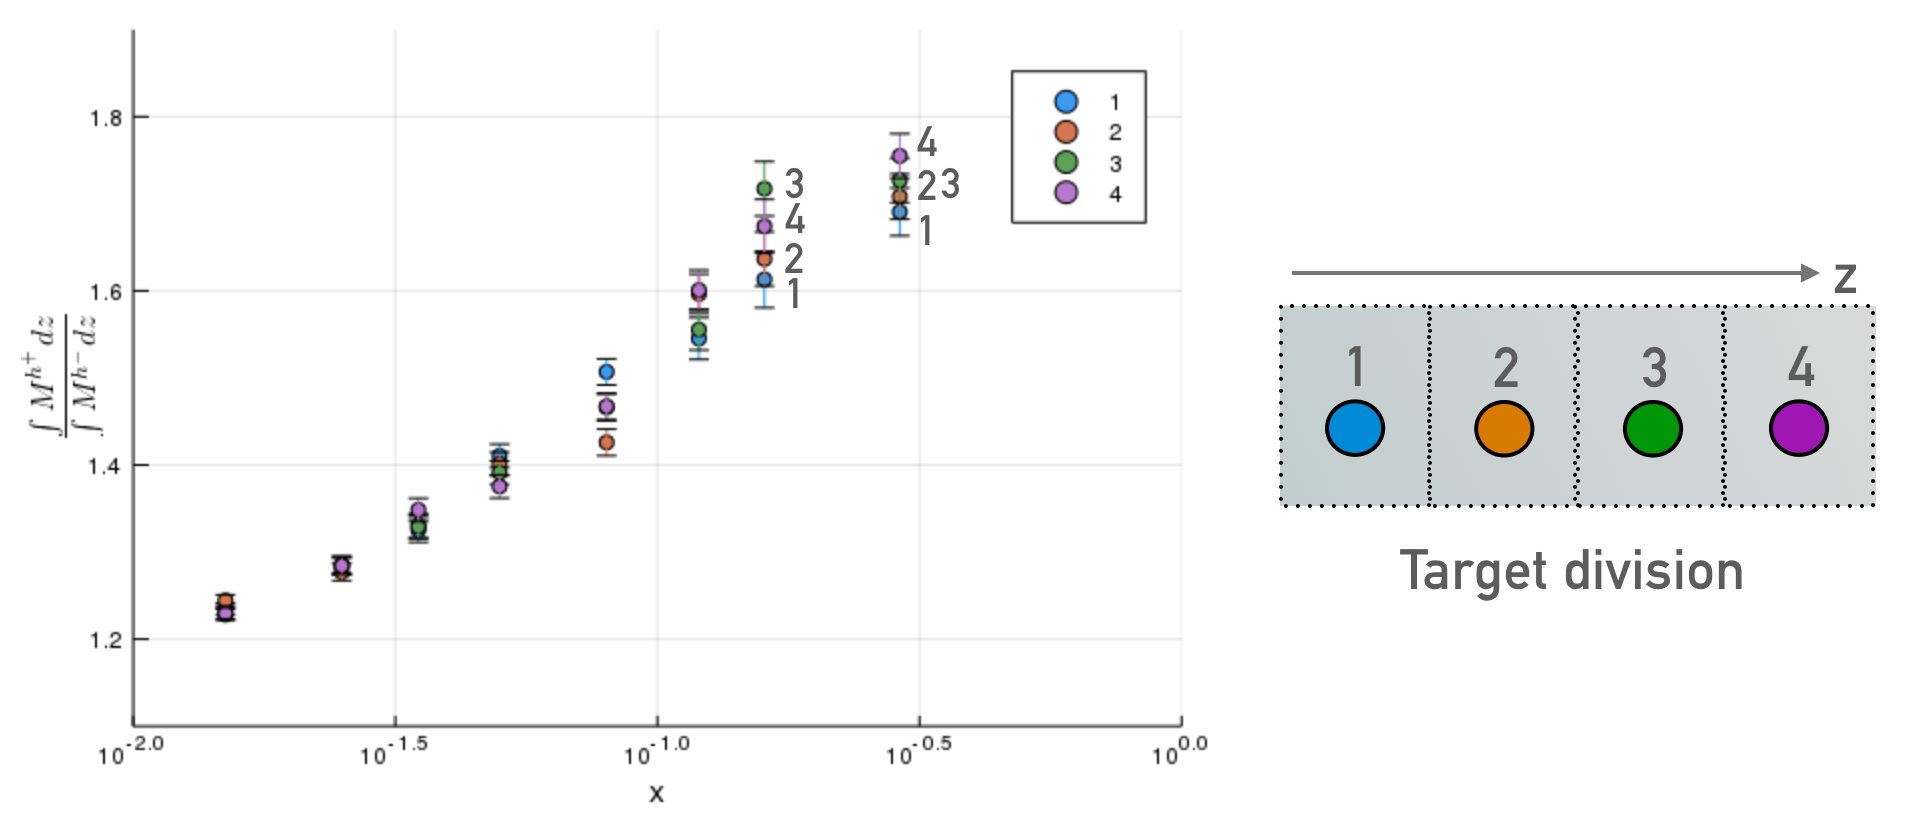
\includegraphics[scale=0.5]{./gfx/RatioVertex.png}}
	\caption{Comparison of the multiplicity sum (a) and ratio (b) for different }
	\label{pic:Zvertexsum}
\end{figure}

In the end, a total systematic uncertainty of $\sim$ 10\% is put on the acceptance.

%------------------------------------------------

\subsection{Systematic uncertainty associated to the diffractive vector meson correction}

In HEPGEN, the cross section for exclusive vector meson production is normalized to the GPD model of Goloskokov and Kroll. The theoretical uncertainty on the predicted cross section close to COMPASS kinematics is around 30\% \cite{Goloskokov}. Propagating this uncertainty leads to a maximum relative uncertainty below 6\%.
The method for the correction of nuclear effects maily changes the shape of the $p_T^2$ distribution with respect to the diffractive vector meson production on a free nucleon. It assumes that the $p_T^2$-integrated nuclear cross-section per nucleon for exclusive events is the same as the $p_T^2$-integrated nuclear cross section for a free nucleon. According to A. Sandacz \cite{Hepgen}, the systematic uncertainty due to this assumption is of a few percent.

%----------------------------------------------------------------------------------------

\section{Charged hadron multiplicities ($h^{\pm}$,$\pi^{\pm}$,$K^{\pm}$,$p/\bar{p}$)}

The multiplicities presented in the following sections include all corrections presented before viz. :

\begin{equation}
  	M^h_{Final}(x,y,z) = M^h_{raw}(x,y,z)\frac{\eta^h(x,y,z)}{A^h(x,y,z)}B^h(x,y,z)
\end{equation}

The $x$,$y$ and $z$ binning is given in Table. \ref{tab:kinbinning}. $A^h$ corresponds to the acceptance correction (Section. \ref{sec:Acc}), $\eta^h$ to the radiative correction factor (Section. \ref{sec:rcf}) and $B^h$ to the diffractive vector meson correction factor (Section. \ref{sec:DVMf}). The statistical error propagation is performed assuming that all corrections are independent :

\begin{equation}
\begin{split}
		E^2_{Final} = \bigg( \frac{RC.VM}{Acc} \bigg)^2 E^2_{Raw} + \bigg(\frac{RC.VM.Raw}{Acc^2} \bigg)^2 E^2_{Acc} \\
		+ \bigg(\frac{RC.Raw}{Acc} \bigg)^2 E^2_{VM} + \bigg(\frac{VM.Raw}{Acc} \bigg)^2 E^2_{RC}
\end{split}
\end{equation}

The corresponding systematic uncertainties from the different sources are added quadratically. The largest contribution in most bins comes from the systematic uncertainty on the acceptance.

\subsection{Unidentified charged hadron multiplicities}

The unidentified charged hadron multiplicities $M^{h^{\pm}}$ are shown in Fig. \ref{pic:mhp} and \ref{pic:mhm} as a function of $z$, in bins of $x$ and staggered vertically with $y$. A strong $z$ dependence is observed for all ($x$,$y$) bins as well as a small dependence with $x$. The $Q^2$ values are in the range 1 to 30 (GeV/$c$)$^2$. $M^{h^+}$ and $M^{h^-}$ have 300 data points each. The statistical uncertainties are too small to be visible in almost all kinematic bins. The bands at the bottom of each $x$ bin panel are the systematic errors for the bin 0.3$< y <$0.5 (bin that covers the largest $z$ range). They are very similar but not shown for the other $y$ bins.

\begin{figure}[!h]
  \centering
	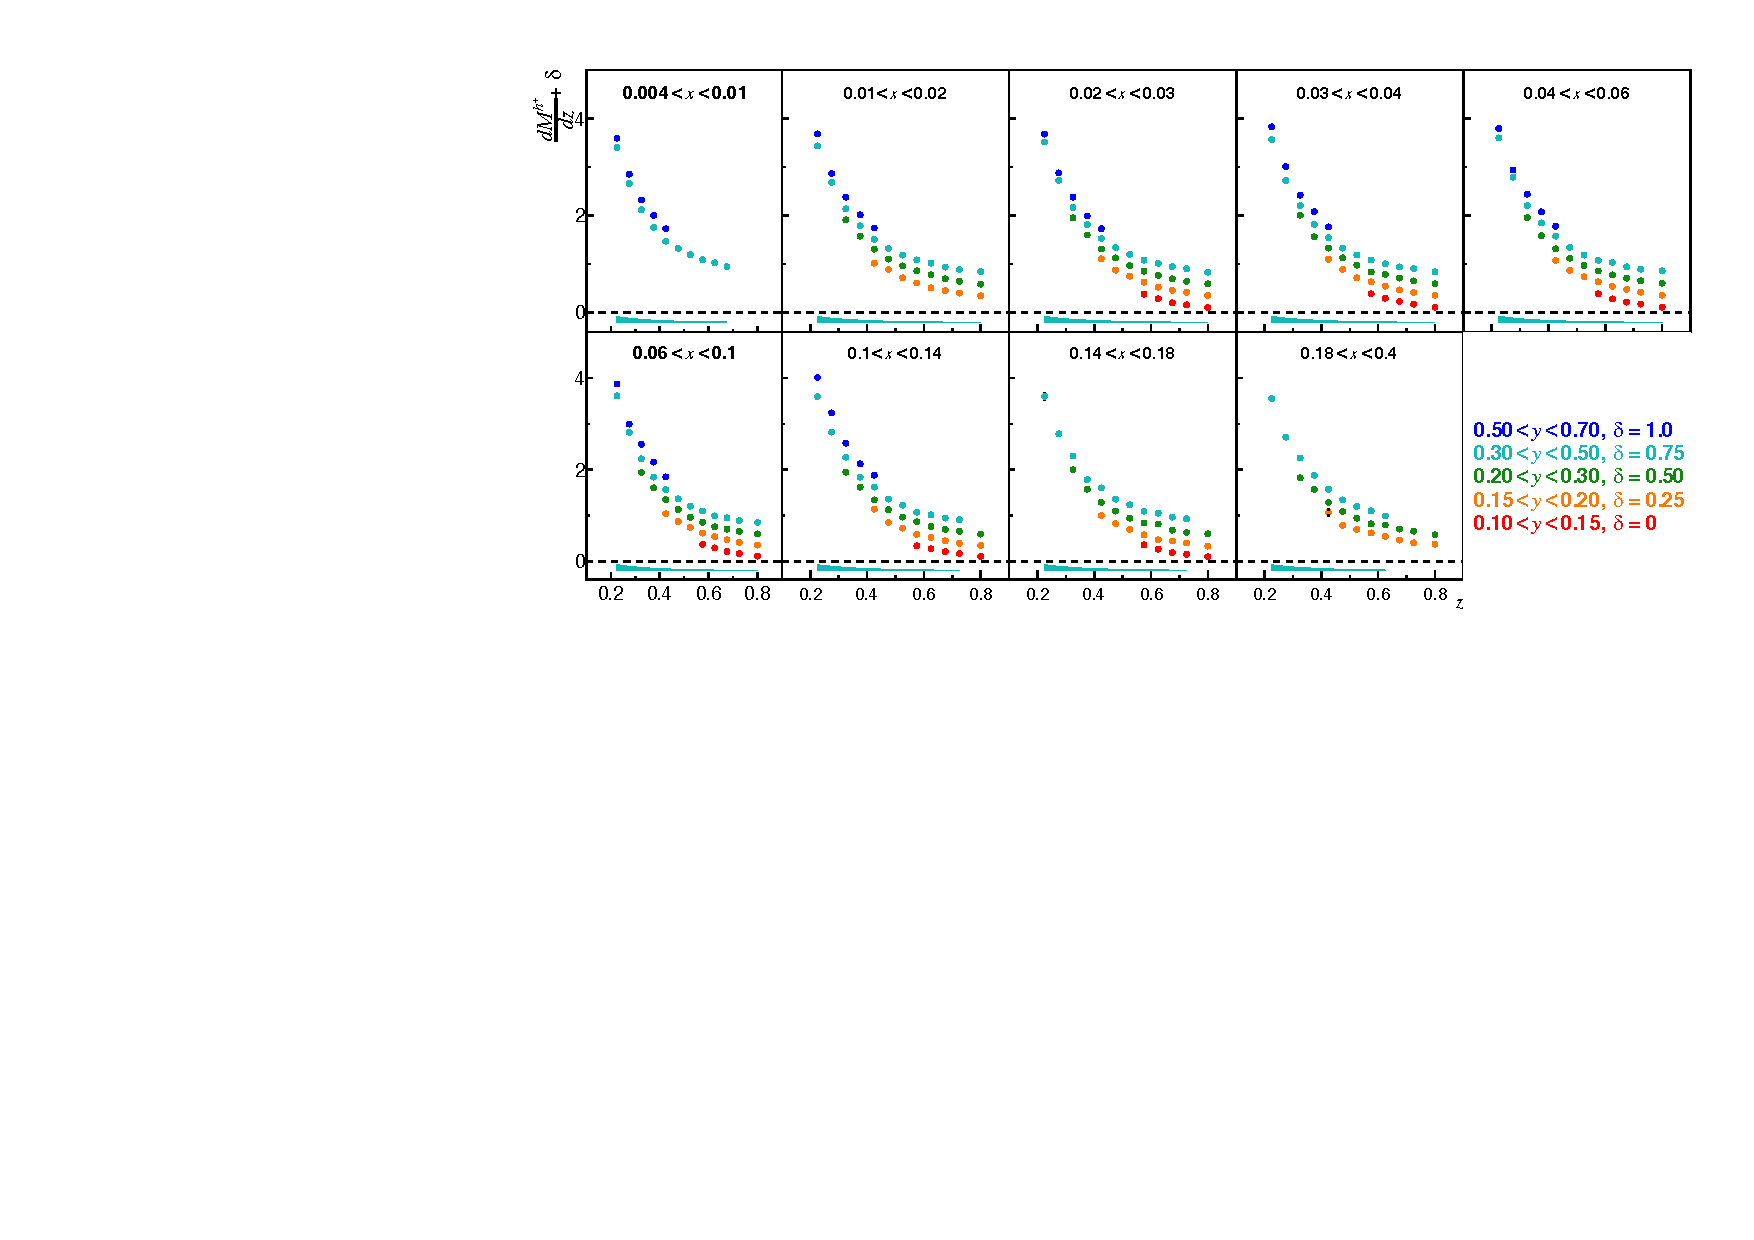
\includegraphics[scale=0.85]{./gfx/hp.pdf}
	\caption{Unidentified positive hadron multiplicities (with all corrections) as a function of $z$ in bins of $x$ staggered vertically with $y$.}
	\label{pic:mhp}
\end{figure}

\begin{figure}[!h]
  \centering
	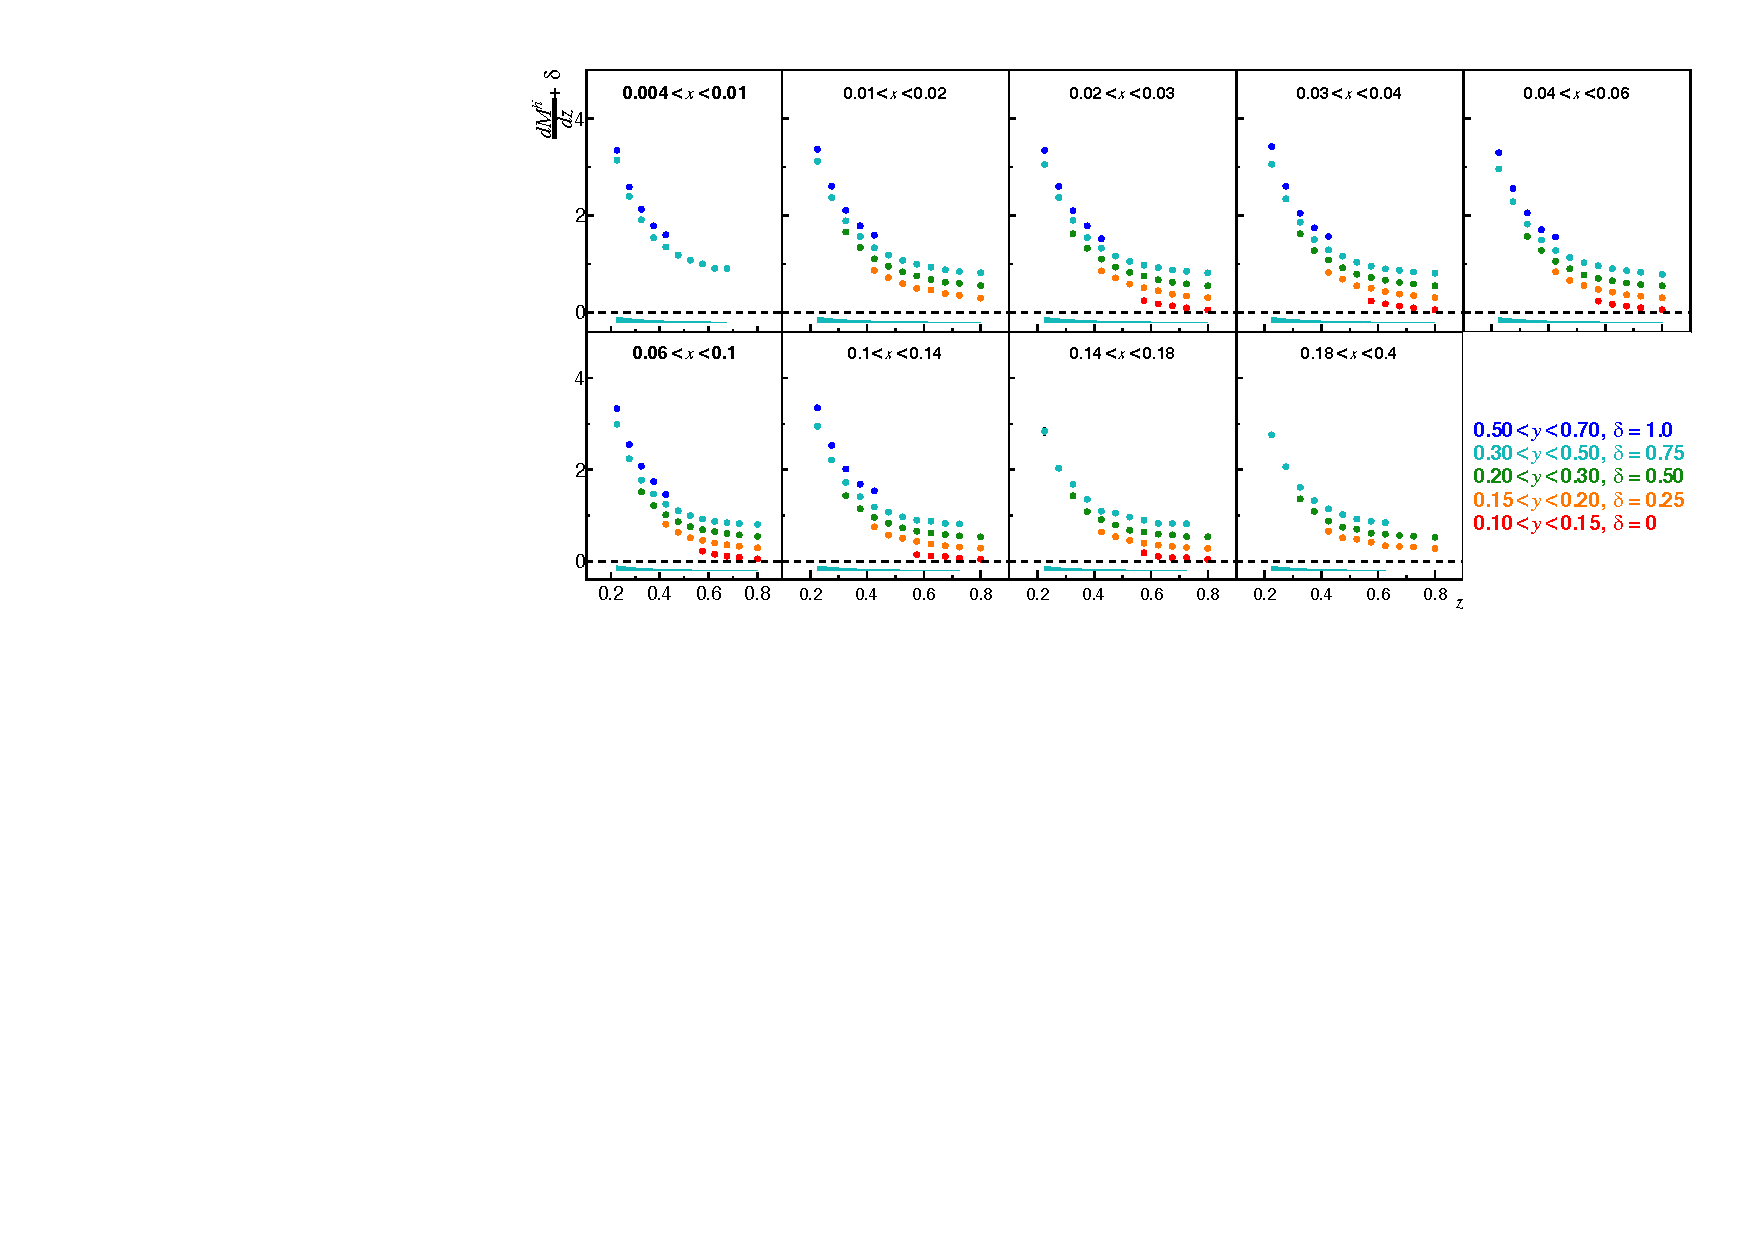
\includegraphics[scale=0.85]{./gfx/hm.pdf}
	\caption{Unidentified positive hadron multiplicities (with all corrections) as a function of $z$ in bins of $x$ staggered vertically with $y$.}
	\label{pic:mhm}
\end{figure}

When removing the $y$ staggering on the previous results, one can see that all data points for different $y$ bins are overlapping (Fig. \ref{pic:mhnoy}). That means that our multiplicities results have no $y$ dependence and can then be averaged over $y$, using the square of the statistical error as weight. Then the multiplicities are displayed as a function of $z$ and in bins of $x$. With Fig. \ref{pic:mhyavg} an asymmetry between $h^+$ and $h^-$ is observed, increasing with $x$.

\begin{figure}[!h]
  \centering
	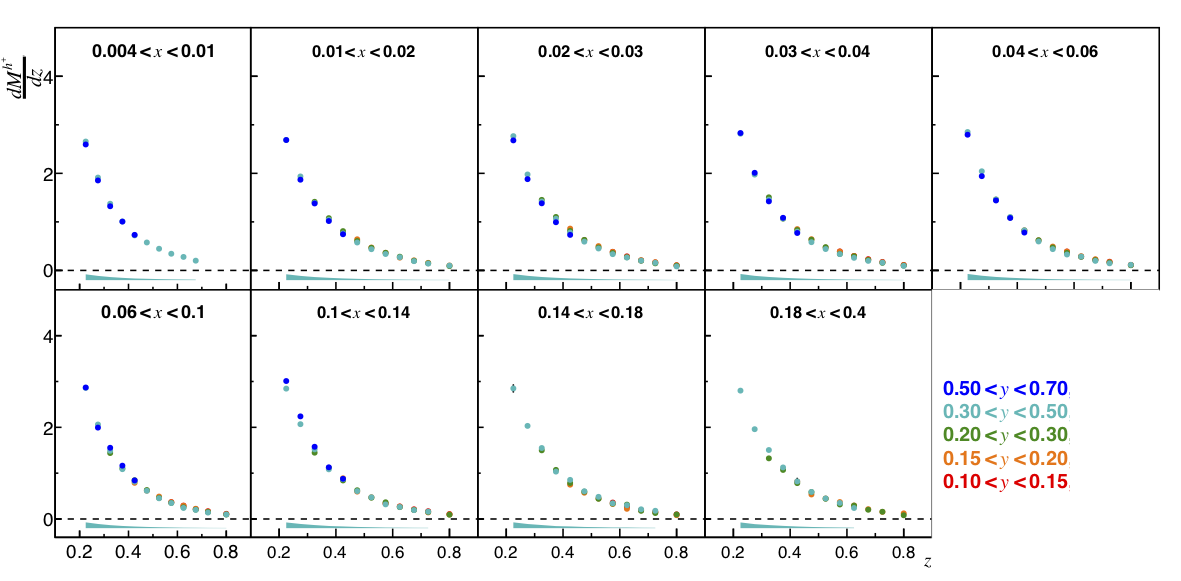
\includegraphics[scale=0.85]{./gfx/hnoystag.png}
	\caption{Unidentified positive hadron multiplicities (with all corrections) as a function of $z$ in bins of $x$. The vertical staggering with $y$ has been suppressed showing that the different $y$ bins do overlap.}
	\label{pic:mhnoy}
\end{figure}

\begin{figure}[!h]
  \centering
	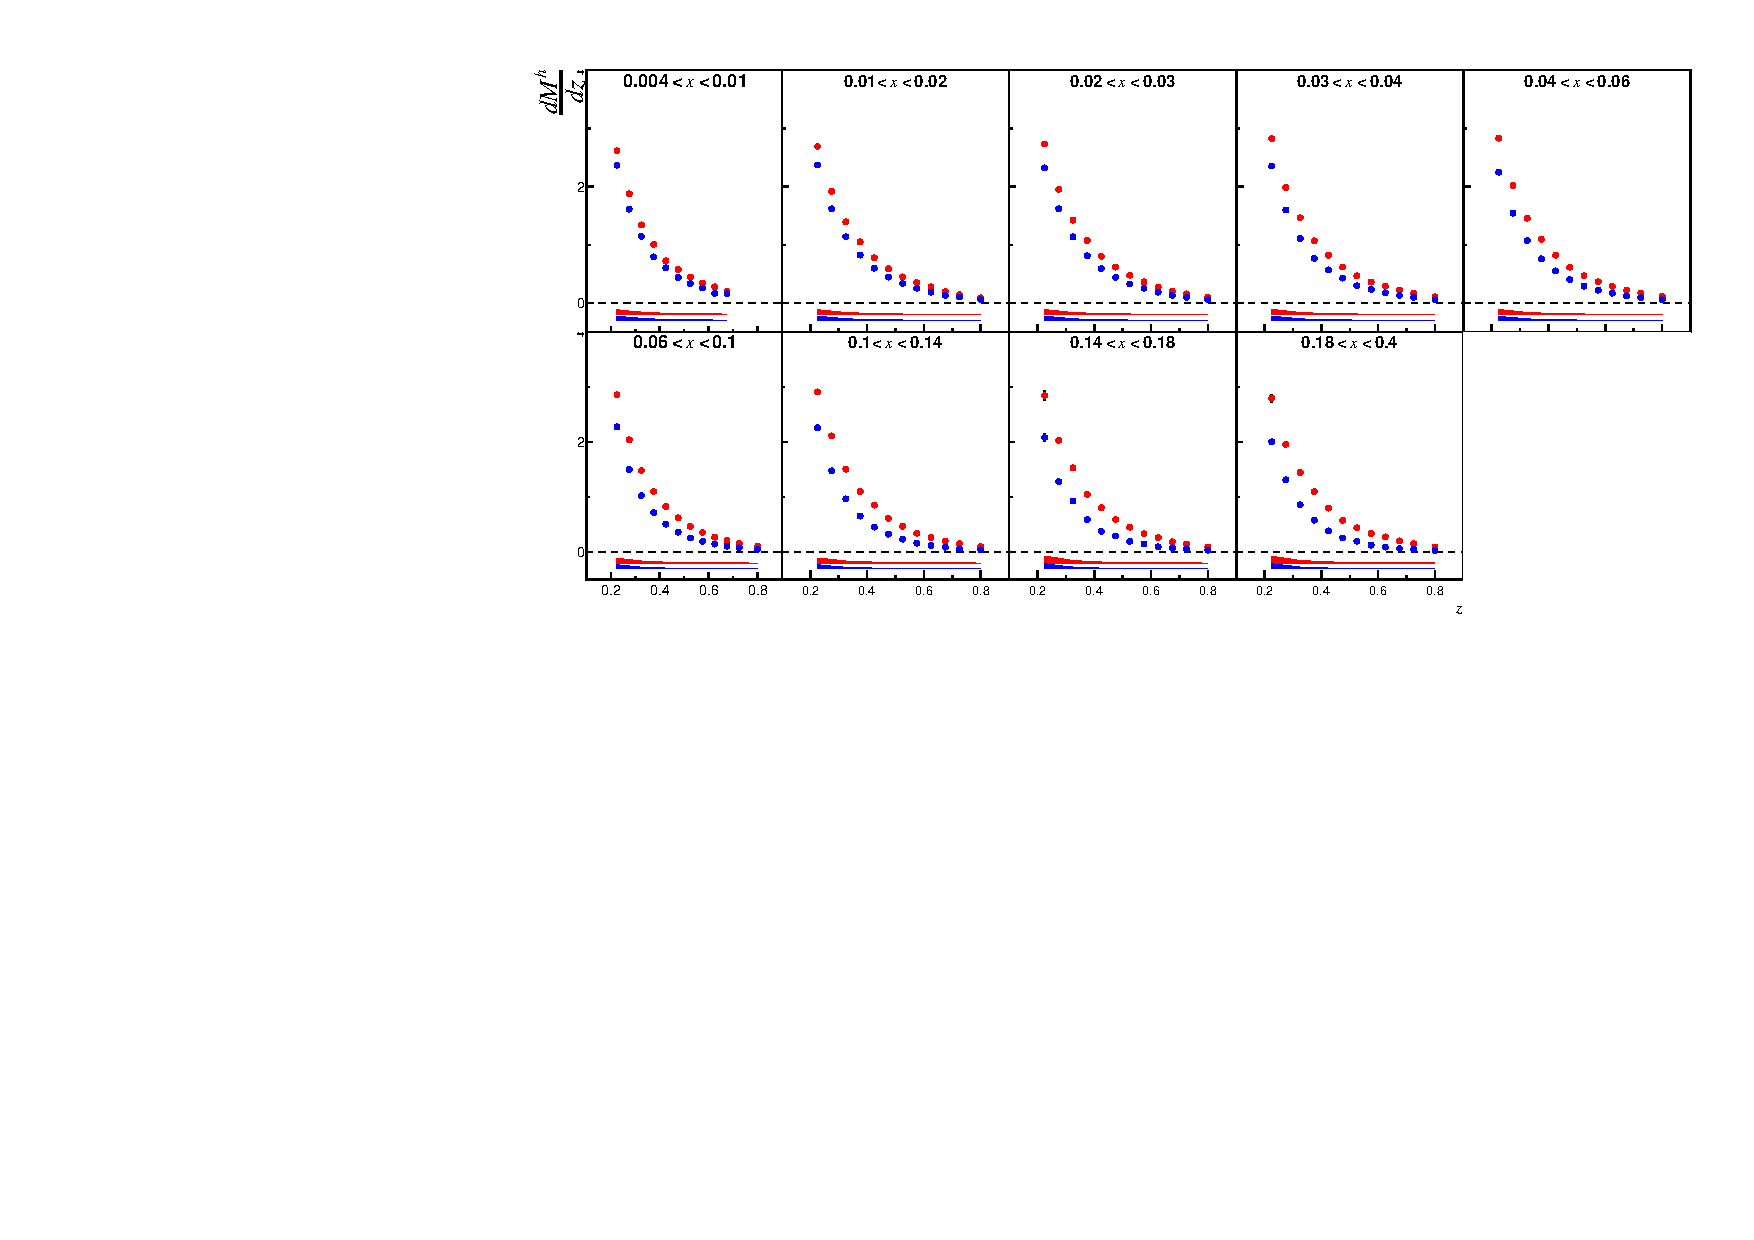
\includegraphics[scale=0.85]{./gfx/hyavg.pdf}
	\caption{Unidentified positive (red) and negative (blue) hadron multiplicities (with all corrections) averaged over $y$ as a function of $z$ in bins of $x$.}
	\label{pic:mhyavg}
\end{figure}

\newpage

\subsection{Charged pion multiplicities}

The charged pion multiplicities $M^{\pi^{\pm}}$ are shown in Fig. \ref{pic:mpip} and \ref{pic:mpim} as a  function of $z$, in bins of $x$ and staggered vertically with $y$. A strong $z$ dependence is observed for all ($x$,$y$) bins as well as a small dependence with $x$. $M^{\pi^+}$ and $M^{\pi^-}$ have 300 data points each. The statistical uncertainties are too small to be visible in almost all kinematic bins. The bands at the bottom of each $x$ bin panel are the systematic errors for the bin 0.3$< y <$0.5 (bin that covers the largest $z$ range).

\begin{figure}[!h]
  \centering
	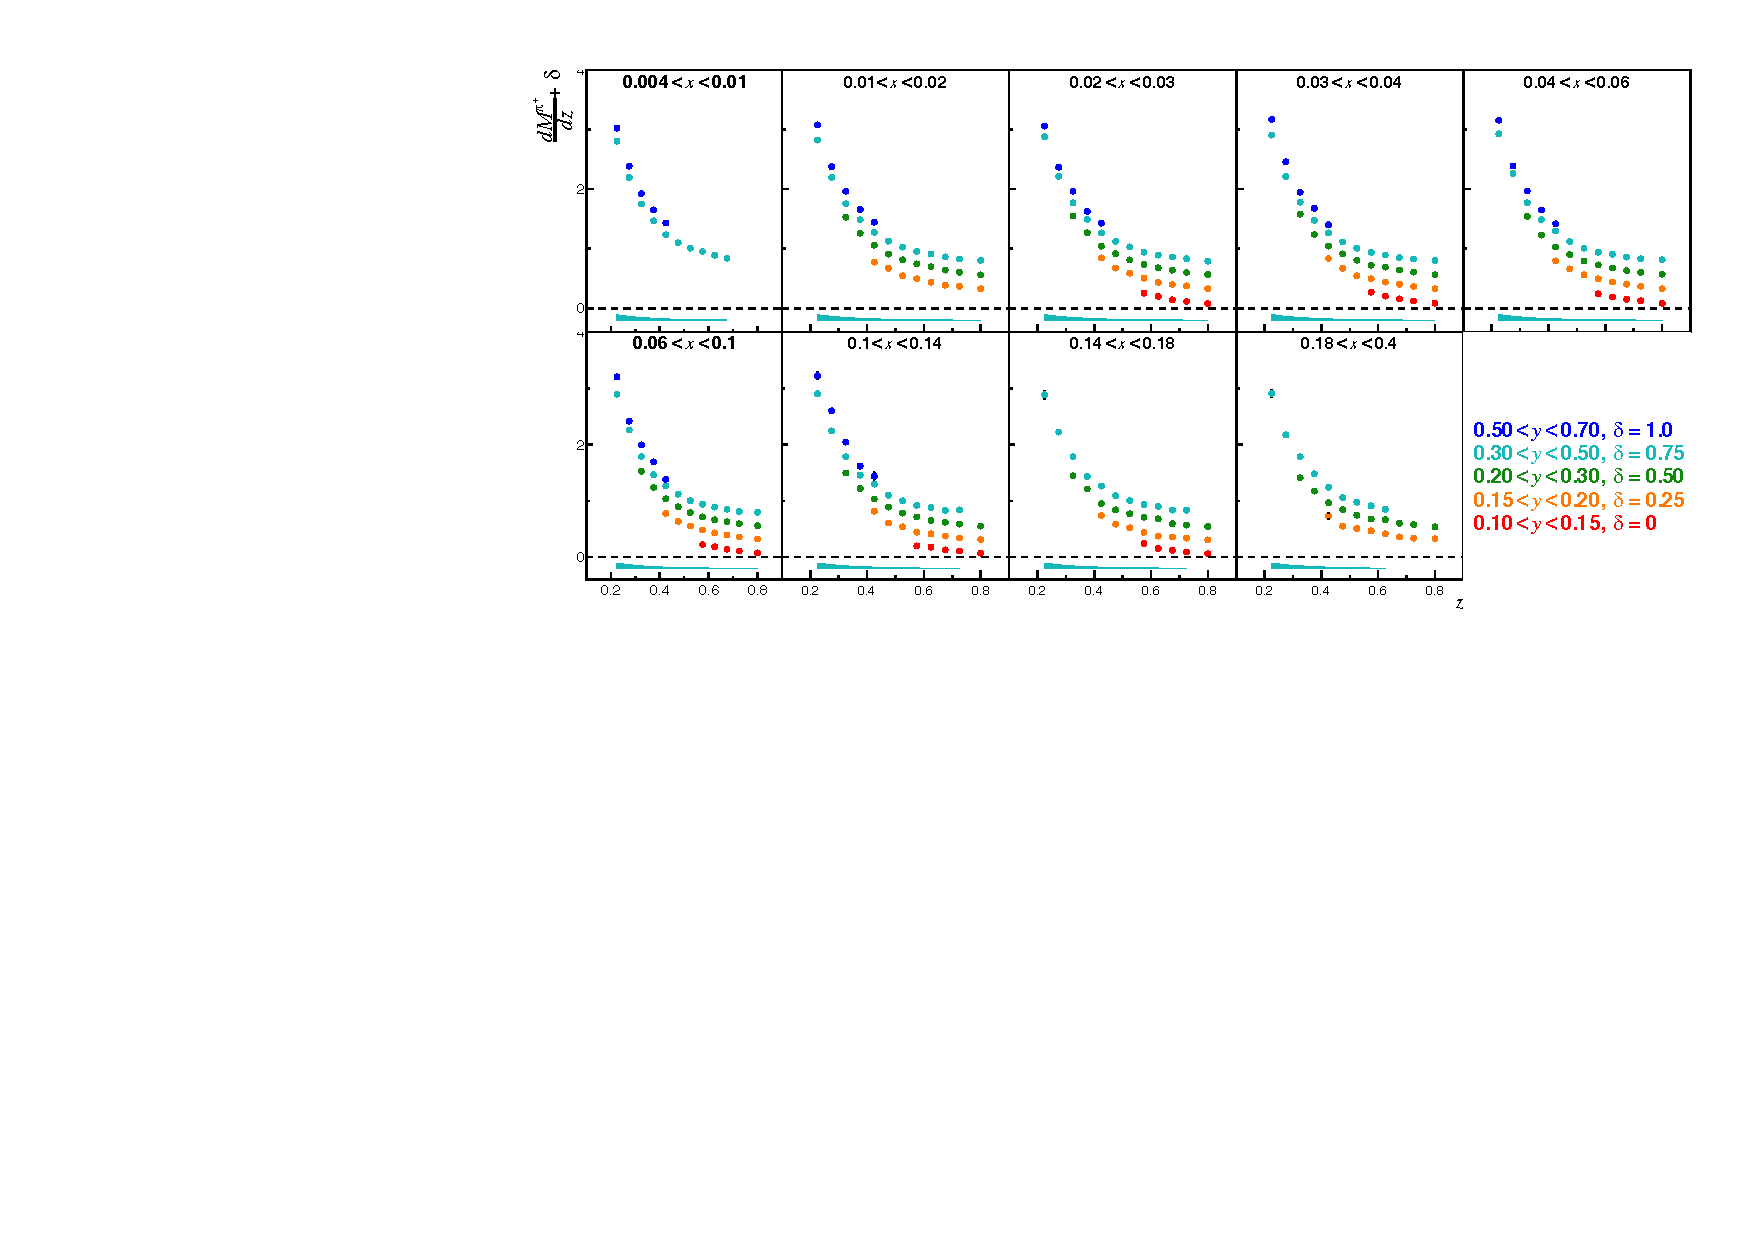
\includegraphics[scale=0.85]{./gfx/pip.pdf}
	\caption{Positive pion multiplicities (with all corrections) as a function of $z$ in bins of $x$, staggered vertically with $y$.}
	\label{pic:mpip}
\end{figure}

\begin{figure}[!h]
  \centering
	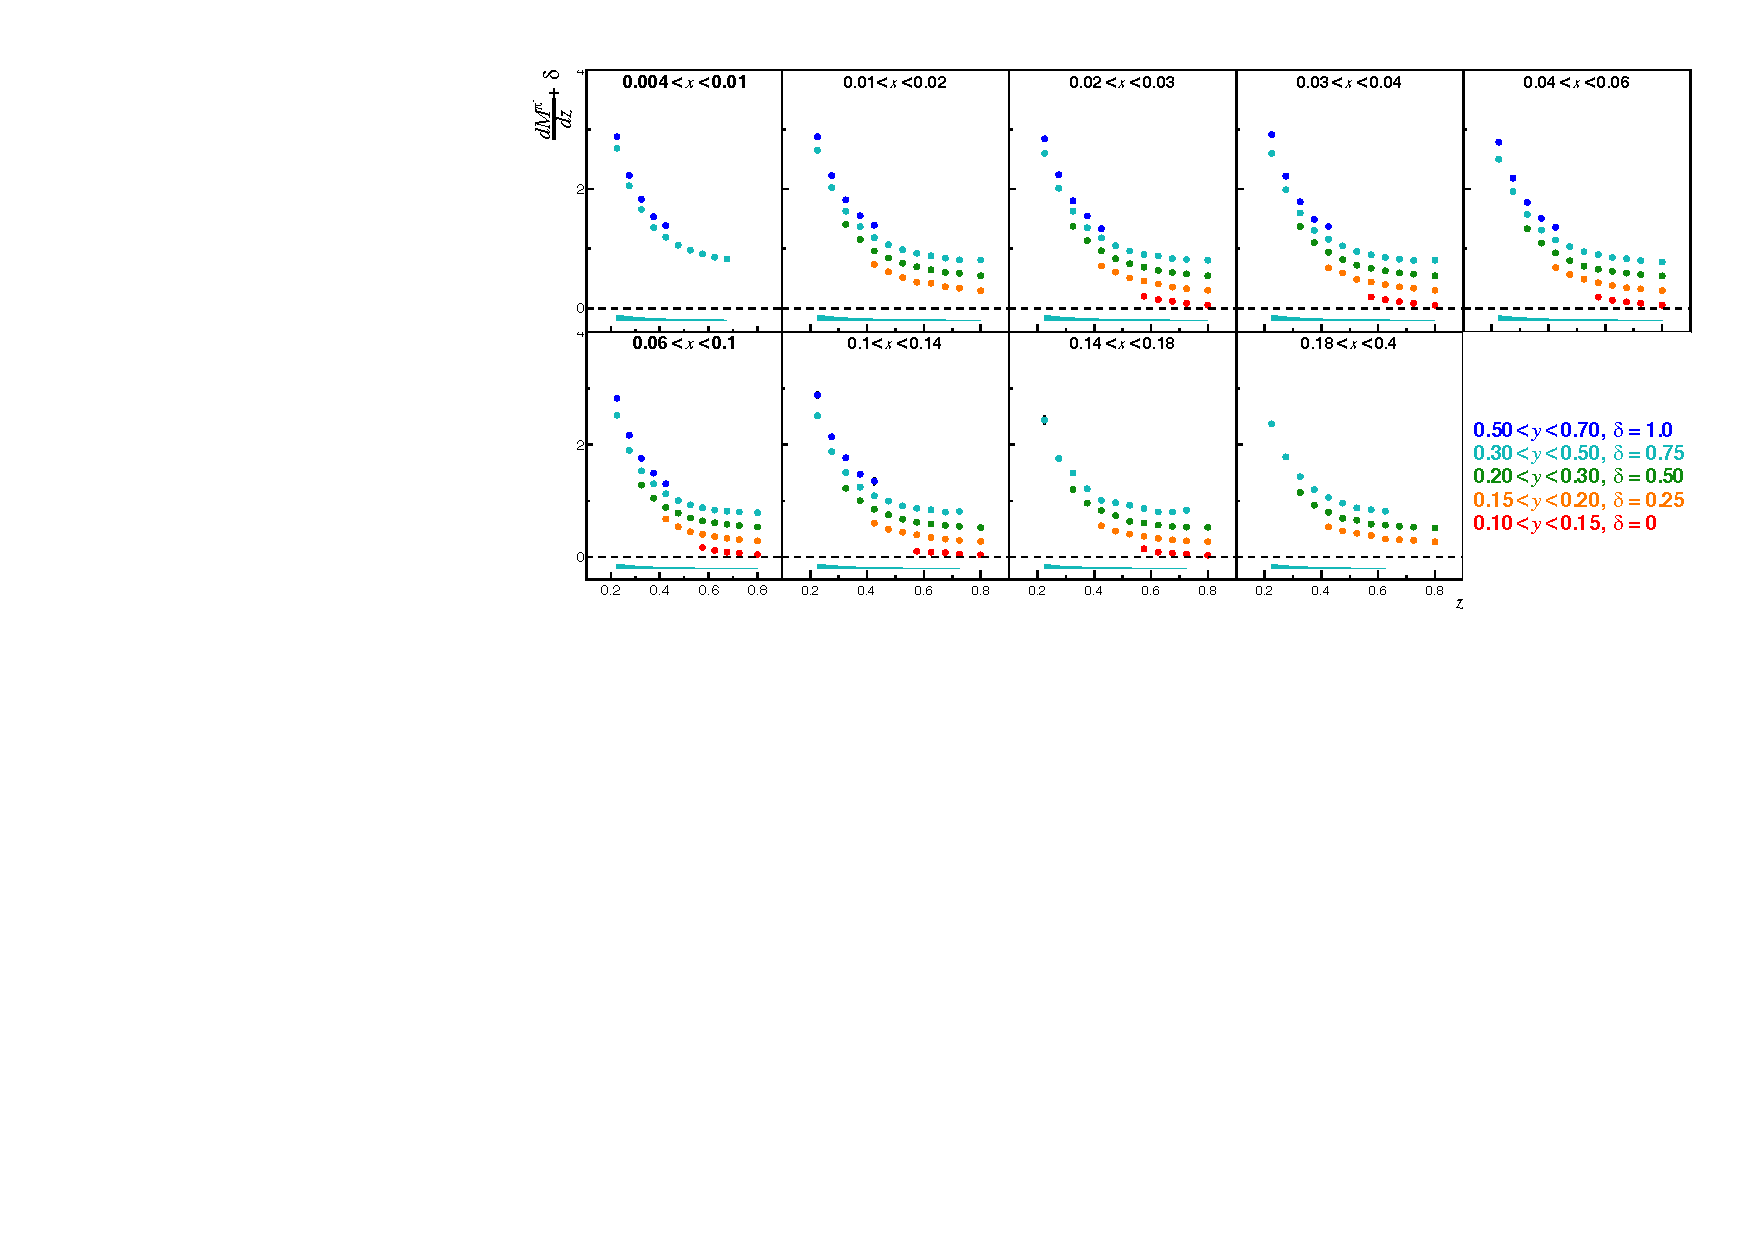
\includegraphics[scale=0.85]{./gfx/pim.pdf}
	\caption{Negative pion multiplicities (with all corrections) as a function of $z$ in bins of $x$, staggered vertically with $y$.}
	\label{pic:mpim}
\end{figure}

The y-averaged multiplicities are displayed as a function of $z$ and in bins of $x$. With Fig. \ref{pic:mpiyavg} an asymmetry between $\pi^+$ and $\pi^-$ is observed, increasing with $x$. Having more $\pi^+$ than $\pi^-$ is due to the fact there is a dominant $u$ quark distribution in the target.

\begin{figure}[!h]
  \centering
	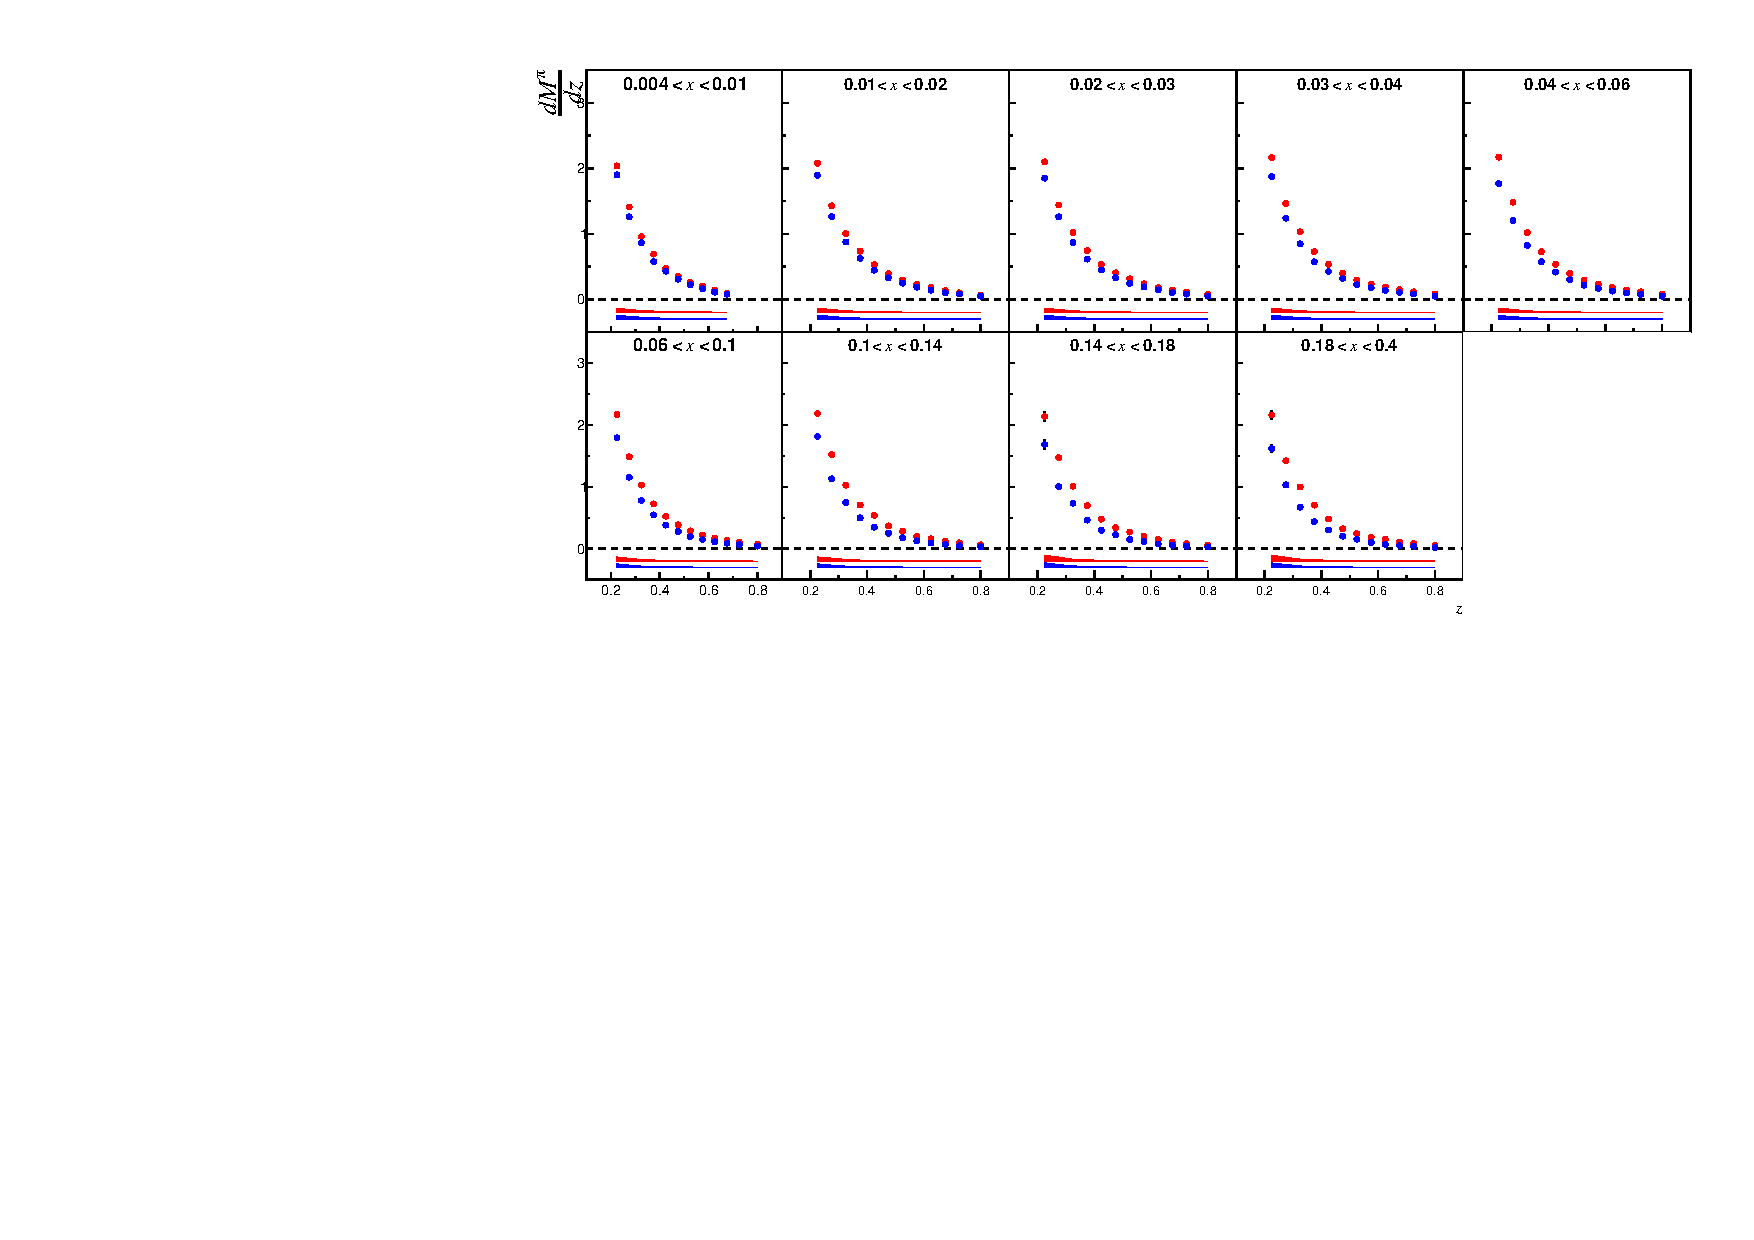
\includegraphics[scale=0.85]{./gfx/piyavg.pdf}
	\caption{Positive (red) and negative (blue) pion multiplicities (with all corrections) averaged over $y$ as a function of $z$ in bins of $x$.}
	\label{pic:mpiyavg}
\end{figure}

\newpage

\subsection{Charged kaon multiplicities}

The charged kaon multiplicities $M^{K^{\pm}}$ are shown in Fig. \ref{pic:mpip} and \ref{pic:mpim} as a function of $z$, in bins of $x$ and staggered vertically with $y$. A strong $z$ dependence is observed for all ($x$,$y$) bins as well as a small dependence with $x$. $M^{K^+}$ and $M^{K^-}$ have 300 data points each. The statistical uncertainties are too small to be visible in almost all kinematic bins. The bands at the bottom of each $x$ bin panel are the systematic errors for the bin 0.3$< y <$0.5 (bin that covers the largest $z$ range).

\begin{figure}[!h]
  \centering
	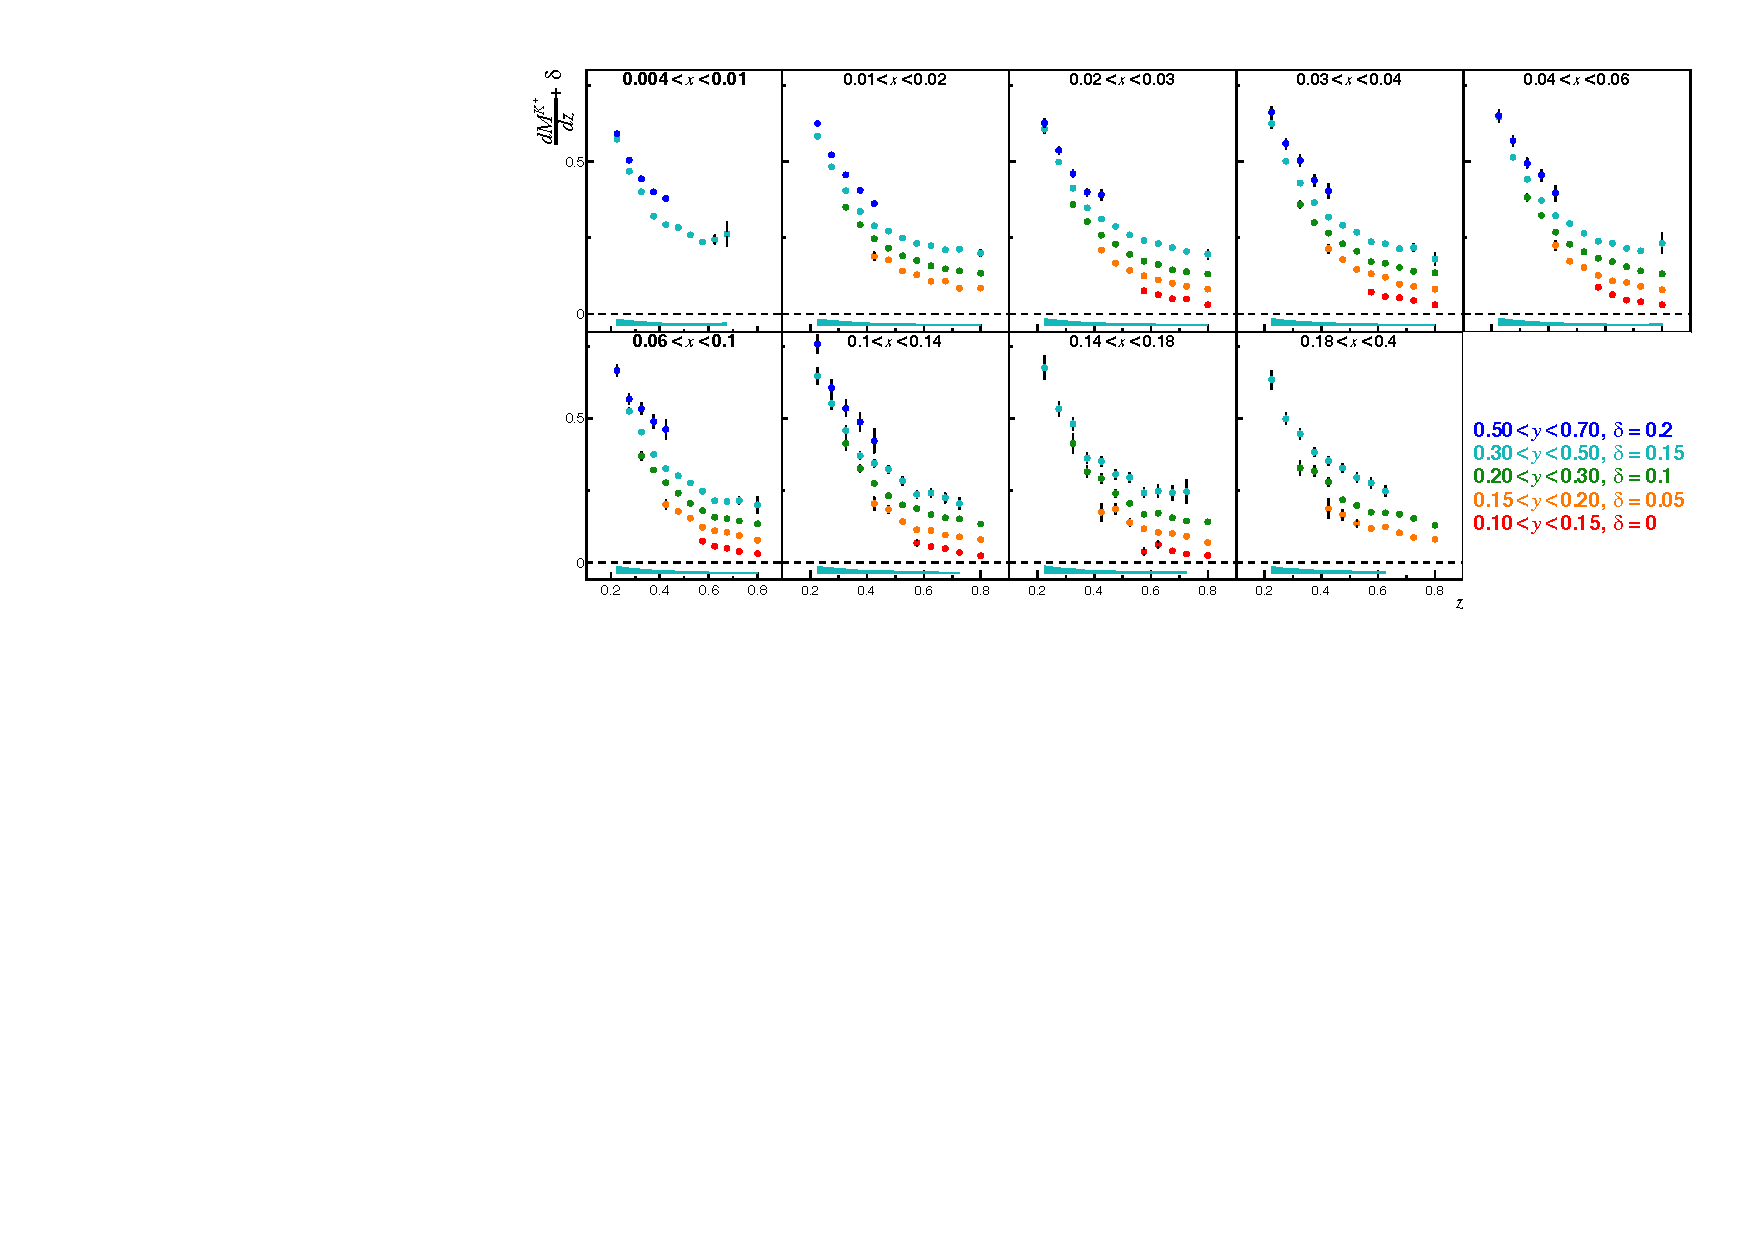
\includegraphics[scale=0.85]{./gfx/Kp.pdf}
	\caption{Positive kaon multiplicities (with all corrections) as a function of $z$ in bins of $x$, staggered vertically with $y$.}
	\label{pic:mkp}
\end{figure}

\begin{figure}[!h]
  \centering
	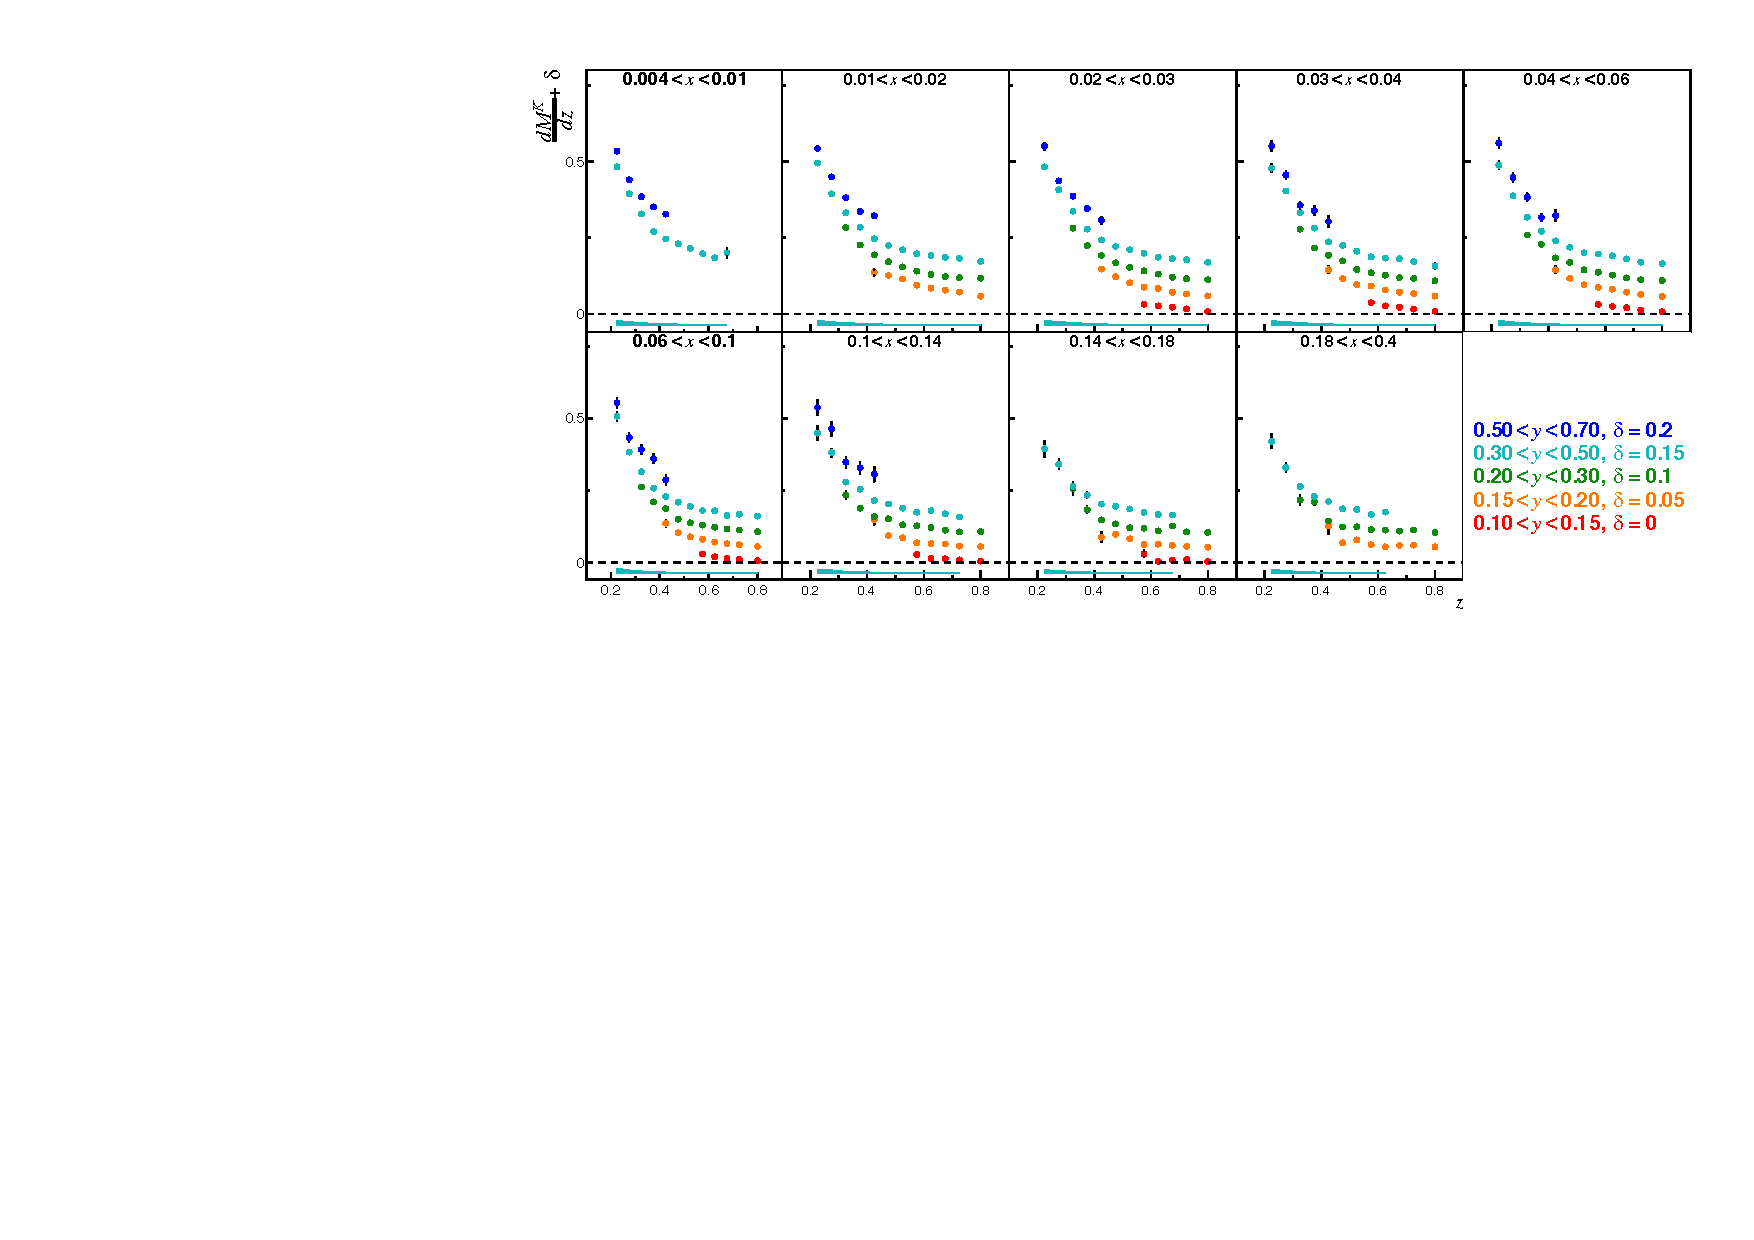
\includegraphics[scale=0.85]{./gfx/Km.pdf}
	\caption{Negative kaon multiplicities (with all corrections) as a function of $z$ in bins of $x$, staggered vertically with $y$.}
	\label{pic:mkm}
\end{figure}

The y-averaged multiplicities are displayed as a function of $z$ and in bins of $x$. With Fig. \ref{pic:mkyavg} an asymmetry between $K^+$ and $K^-$ is observed, increasing with $x$. Having more $K^+$ than $K^-$ is due to the fact there is a dominant $u$ quark distribution in the target. In addition, producing $K^-$ requires sea quarks only.

\begin{figure}[!h]
  \centering
	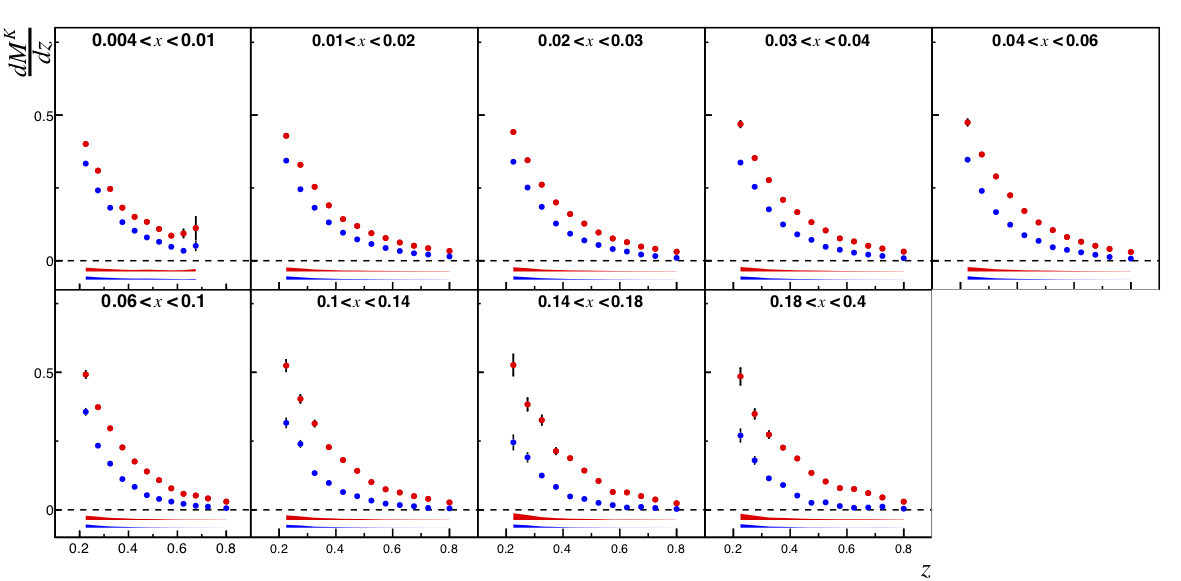
\includegraphics[scale=0.85]{./gfx/Kyavg.png}
	\caption{Positive (red) and negative (blue) kaon multiplicities (with all corrections) averaged over $y$ as a function of $z$ in bins of $x$.}
	\label{pic:mkyavg}
\end{figure}

\newpage

\subsection{Proton/Antiproton multiplicities}

The proton/antiproton multiplicities $M^{p/\bar{p}}$ are shown in Fig. \ref{pic:mpp} and \ref{pic:mpm} as a function of $z$, in bins of $x$ and staggered vertically with $y$. A strong $z$ dependence is observed for all ($x$,$y$) bins as well as a small dependence with $x$. $M^{K^+}$ and $M^{K^-}$ have 300 data points each. The statistical uncertainties are too small to be visible in almost all kinematic bins. The bands at the bottom of each $x$ bin panel are the systematic errors for the bin 0.3$< y <$0.5 (bin that covers the largest $z$ range).

\begin{figure}[!h]
  \centering
	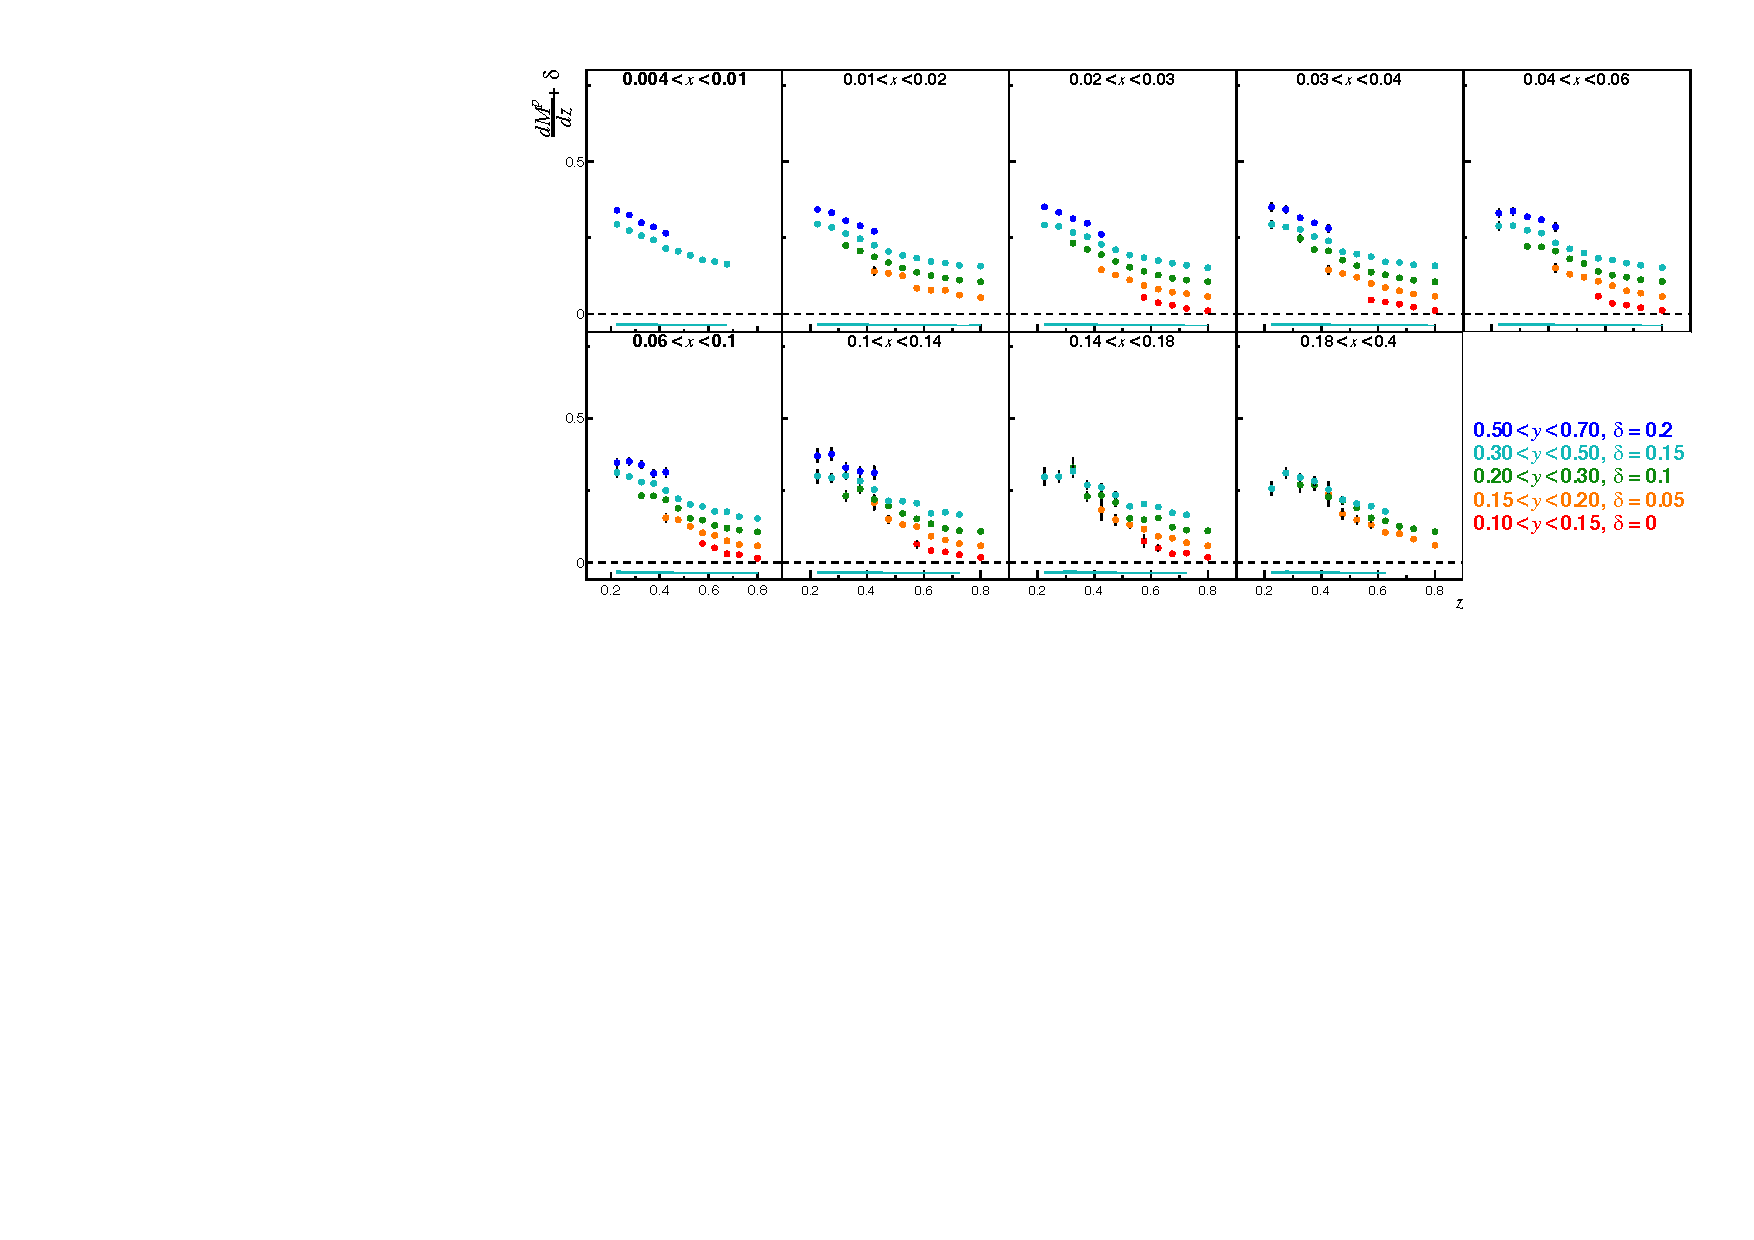
\includegraphics[scale=0.85]{./gfx/pp.pdf}
	\caption{Proton multiplicities (with all corrections) as a function of $z$ in bins of $x$, staggered vertically with $y$.}
	\label{pic:mpp}
\end{figure}

\begin{figure}[!h]
  \centering
	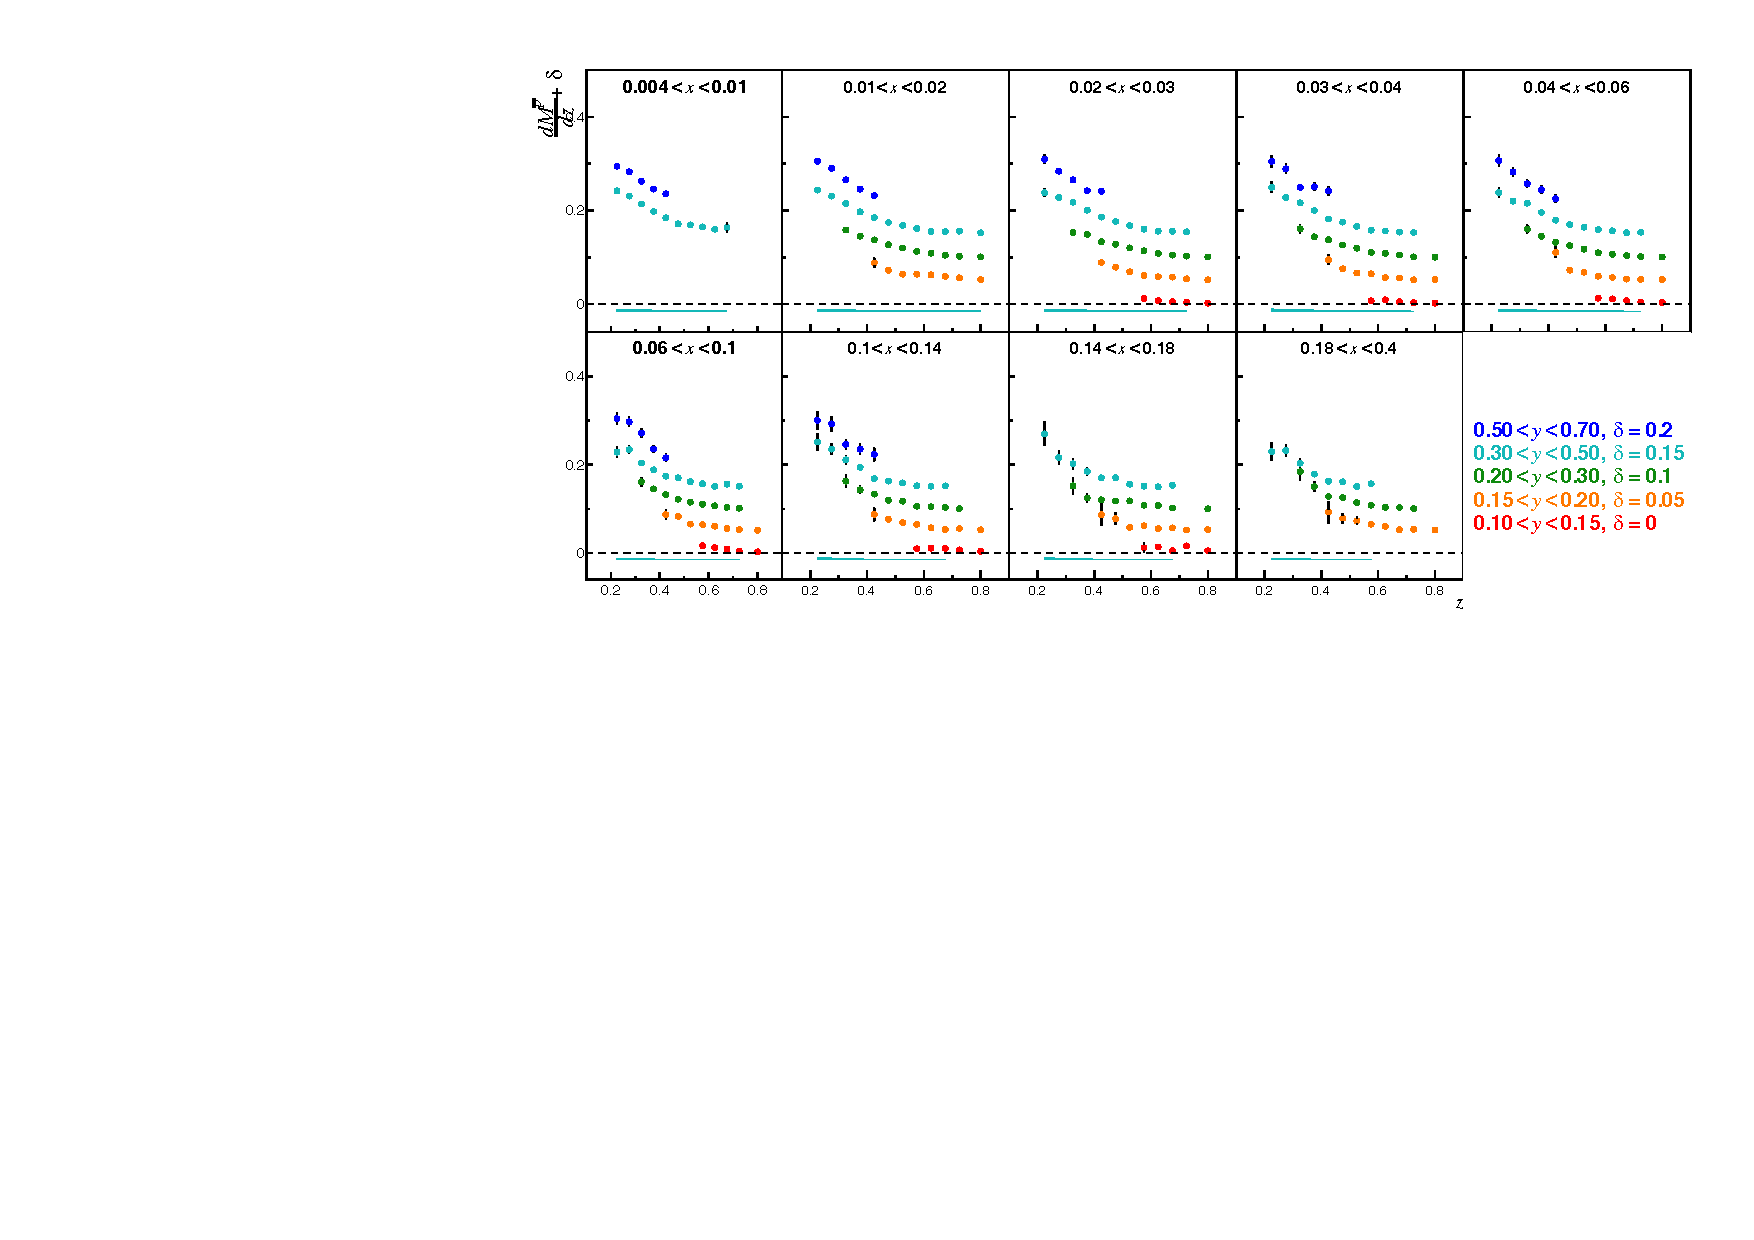
\includegraphics[scale=0.85]{./gfx/pm.pdf}
	\caption{Antiproton multiplicities (with all corrections) as a function of $z$ in bins of $x$, staggered vertically with $y$.}
	\label{pic:mpm}
\end{figure}

The y-averaged multiplicities are displayed as a function of $z$ and in bins of $x$. With Fig. \ref{pic:mpyavg} an asymmetry between $p$ and $\bar{p}$ is observed, increasing with $x$. Having more protons than antiproton is due to the fact there is a dominant $u$ quark distribution in the target. In addition, producing antiprotons requires sea quarks only.

\begin{figure}[!h]
  \centering
	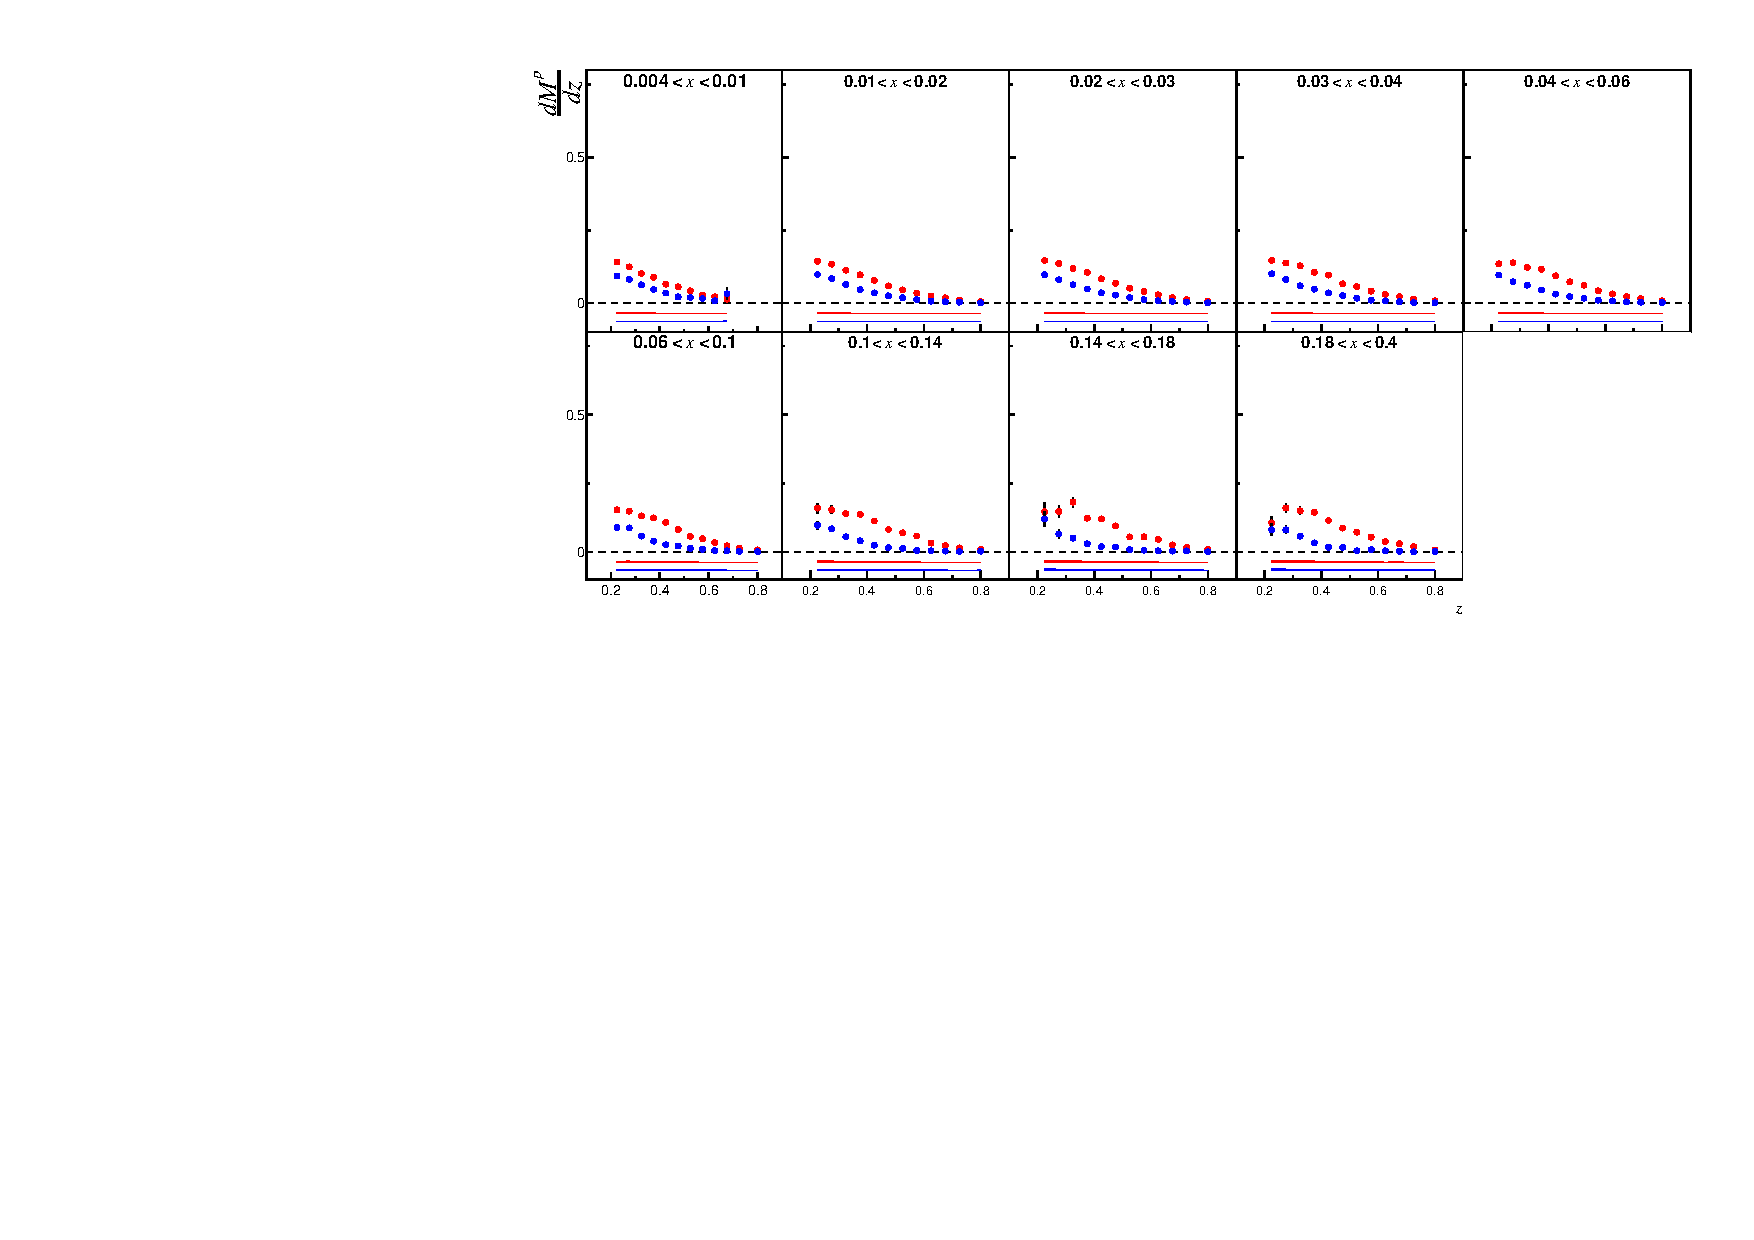
\includegraphics[scale=0.85]{./gfx/pyavg.pdf}
	\caption{Proton (red) and antiproton (blue) multiplicities (with all corrections) averaged over $y$ as a function of $z$ in bins of $x$.}
	\label{pic:mpyavg}
\end{figure}

\newpage

\section{Ratio of charged hadron multiplicities}

From the $y$-averaged multiplicities, we can still integrate on $z$ to get rid of the $z$ dependence, be able to compare our results with other experiment and also have a scent of the underlying physics. One interesting quantity to look at is the ratio of charged hadron multiplicities as with this quantity most of the systematics cancel by and large. The ratio is calculated as following :

\begin{equation}
  \frac{\mathscr{M}^{h^+}}{\mathscr{M}^{h^-}} = \frac{\int_{0.2}^{0.85} \langle M^{h^+} \rangle_y dz}{\int_{0.2}^{0.85} \langle M^{h^-} \rangle_y dz}
\end{equation}

Only the 8 $x$ bins that have a sufficient $z$ coverage subsist.

\subsection{Ratio of unidentified charged hadron multiplicities}

In Fig. \ref{pic:piratio}, the $\mathscr{M}^{h^+}/\mathscr{M}^{h^-}$ from COMPASS is depicted for a proton target (blue points) and for an isoscalar target (orange points).

\begin{figure}[!h]
  \centering
	\includegraphics[scale=0.5]{./gfx/hr.png}
	\caption{Ratio of $\frac{\mathscr{M}^{h^+}}{\mathscr{M}^{h^-}}$ for a proton target (blue closed points) and an isoscalar target (orange closed points) (COMPASS data)}
	\label{pic:hratio}
\end{figure}

The ratio of unidentified charged hadron multiplicity for a proton target should lie above COMPASS results on isoscalar target, the reason being the different quark mixture in the two targets (more $u$ in proton target thus higher $h+$/$h-$ ratio in proton than in isoscalar target). The difference is expected to be $\sim$10-20\%, as obtained here.

\newpage

\subsection{Ratio of charged pion multiplicities}

In Fig. \ref{pic:piratio}, the $\mathscr{M}^{\pi^+}/\mathscr{M}^{\pi^-}$ from COMPASS is depicted for a proton target (blue points) and for an isoscalar target (orange points). The same ratio from HERMES is presented for a proton target (violet open points) and a deuteron target (green open points).

\begin{figure}[!h]
  \centering
	\includegraphics[scale=0.5]{./gfx/pir.png}
	\caption{Ratio of $\frac{\mathscr{M}^{\pi^+}}{\mathscr{M}^{\pi^-}}$ from COMPASS for a proton target (blue closed points) and an isoscalar target (orange closed points) and from HERMES for a proton target (violet open points) and a deuteron target (green open points).}
	\label{pic:piratio}
\end{figure}

For the very same reason as for hadrons, the ratio of charged pions multiplicity for a proton target is expected to be larger than COMPASS results for an isoscalar target by $\sim$10-20\%, as observed here. The COMPASS results for proton and isoscalar targets are compared to HERMES results for proton and deuteron targets. On all the $x$ range, the proton results are compatible within error bars, as were the deuteron results.

\subsection{Ratio of charged kaon multiplicities}

In Fig. \ref{pic:kratio}, the $\mathscr{M}^{K^+}/\mathscr{M}^{K^-}$ from COMPASS is depicted for a proton target (blue points) and for an isoscalar target (orange points). The same ratio from HERMES is presented for a proton target (violet open points) and a deuteron target (green open points).

\begin{figure}[!h]
  \centering
	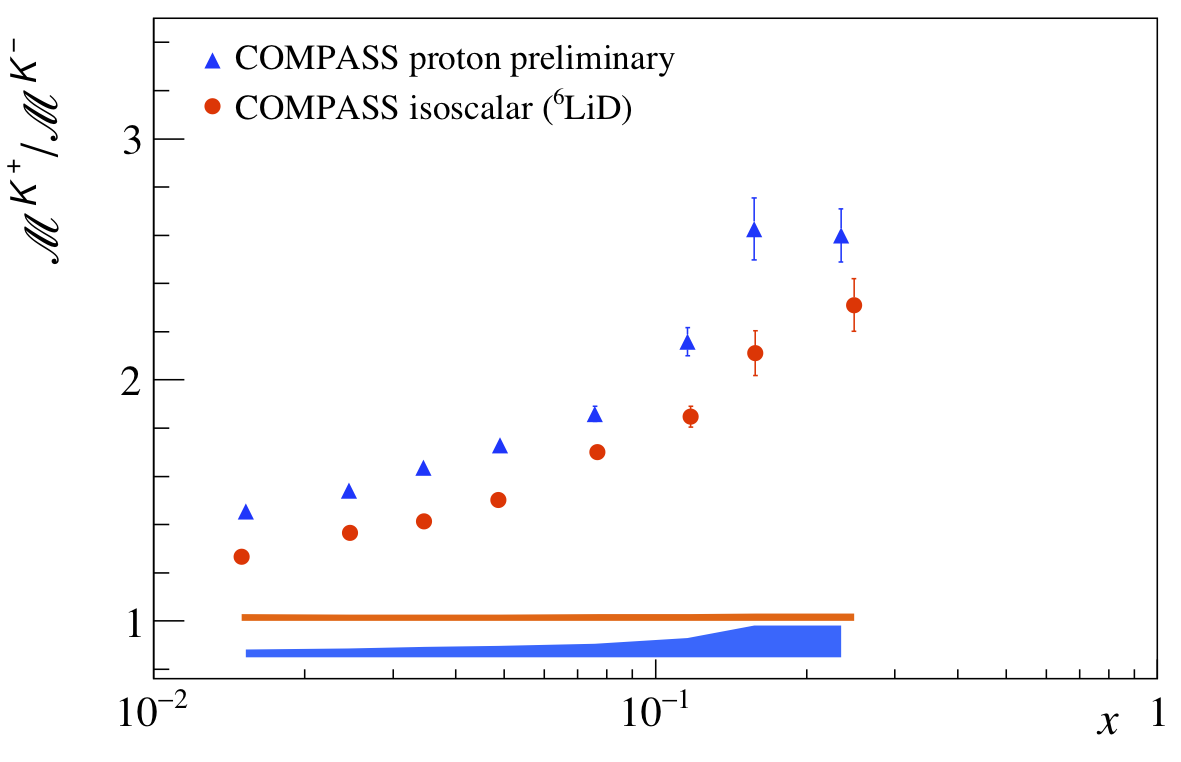
\includegraphics[scale=0.5]{./gfx/Kr_noH.png}
	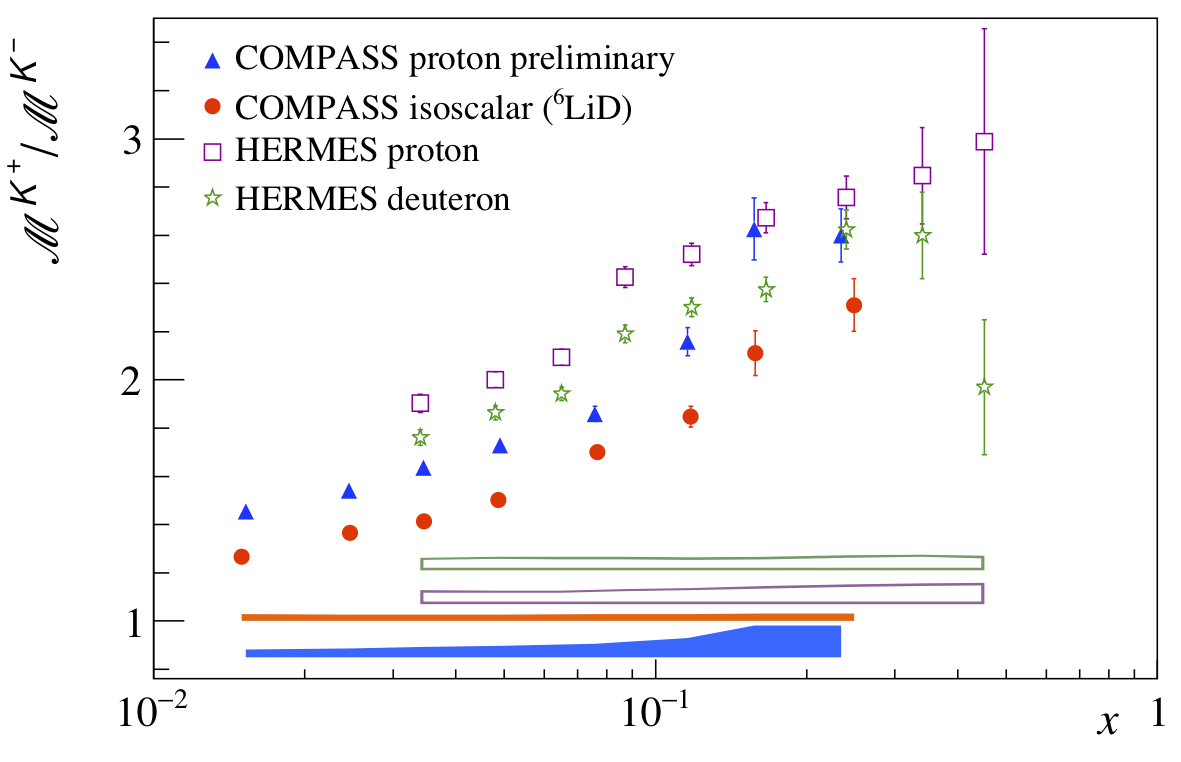
\includegraphics[scale=0.5]{./gfx/Kr.png}
	\caption{Ratio of $\frac{\mathscr{M}^{K^+}}{\mathscr{M}^{K^-}}$ from COMPASS for a proton target (blue closed points) and an isoscalar target (orange closed points) and from HERMES for a proton target (violet open points) and a deuteron target (green open points).}
	\label{pic:kratio}
\end{figure}

For the very same reason as for hadrons and pions, the ratio of charged kaon multiplicity on proton target is expected to be larger than COMPASS results for isoscalar target by $\sim$10\%, as observed here. Contrary to pion case, the comparison of results for the kaon case shows discrepancies between COMPASS and HERMES results for both proton and deuteron/isoscalar targets.

This discrepancy was investigated by the COMPASS collaboration\cite{MarcinPubli}. By defining a missing mass parameter $M_X = \sqrt{M^2_p + 2M_p \nu (1-z) - Q^2 (1-z)^2}$, one can spot that the kaon ratio, especially at $z$ $>$ 0.75, is depending on this parameter. Thus, the ratio is in fact a function of $\nu$ and $z$. The COMPASS results for deuteron target were in tension with pQCD predictions hence pointing to the need of a correction within the pQCD formalism to take into account the phase-space available for the hadronisation of the target remnants. Moreover, for other experiments than COMPASS, deviations may even appear at lower $z$. Coming back to the comparison between COMPASS and HERMES results, when taking data points where there are the exact same kinematics, the results for kaon multiplicities ratio are agreeing, which makes sense at the light of the investigation mentionned before. This explanation might in fact explain at least part of the discrepancy observed between COMPASS and HERMES. Another lead to reconcile the results is to look for hadron mass correction\cite{Accardi}, which also explains part of the discrepancy observed.

\subsection{Ratio of proton/anitproton multiplicities}

In Fig. \ref{pic:pratio}, the $\mathscr{M}^{p}/\mathscr{M}^{\bar{p}}$ from COMPASS is depicted for a proton target (blue points). This is the first time that this quantity is measured.

\begin{figure}[!h]
  \centering
	\includegraphics[scale=0.5]{./gfx/pr.png}
	\caption{Ratio of $\frac{\mathscr{M}^{p}}{\mathscr{M}^{\overline{p}}}$ from COMPASS for a proton target (blue closed points).}
	\label{pic:pratio}
\end{figure}

\section{Sum of charged hadron multiplicities}

An other interesting quantity to look at is the sum of charged hadron multiplicities (e.g. $\mathscr{M}^{h^+}+\mathscr{M}^{h^-}$) as for an isoscalar target, it was easy to interpret this sum for given $x$ values. Unfortunately, such interpretations are not anymore feasible for a proton target. However they are still relevant quantity to compute as for some type of hadrons, the results between the multiplicities extracted on a proton target ($lH_2$, this analysis) and an isoscalar target ($^6LiD$, COMPASS published results) should be similar.

\subsection{Sum of unidentified charged hadron multiplicities}

By integrating over $z$ the charged hadron multiplicities averaged over $y$, one can obtain multiplicities that are only depending on one parameter, $x$. In order to get rid of of the charge dependence of the charged hadron multiplicities, the charged hadron multiplicity sum is studied. In Fig. \ref{pic:hsum}, the $\mathscr{M}^{h^+}+\mathscr{M}^{h^-}$ from COMPASS is depicted for a proton target (blue points) and for an isoscalar target (orange points).

\begin{figure}[!h]
  \centering
	\includegraphics[scale=0.5]{./gfx/hs.png}
	\caption{Sum of $\mathscr{M}^{h^+}+\mathscr{M}^{h^-}$ from COMPASS for a proton target (blue closed points) and an isoscalar target (orange closed points).}
	\label{pic:hsum}
\end{figure}

The sum of charged hadron multiplicity $\mathscr{M}^{h^+}+\mathscr{M}^{h^-}$ for a proton target should lie at the same level than COMPASS results for an isoscalar target. The discrepancy in amplitude can be explained by the fact that the radiative correction at the time of the publication were not correct and with our nowadays knowledge of radiative corrections, we know that all the points should be moved up by $\sim$6\%, which reconciles proton and isoscalar results within error bars, at least for low $x$. At high $x$ for the results on proton target, the problem comes likely from a bad description of semi-inclusive variable in the Monte-Carlo like $\theta_h$. In the 2006 analysis, the high-$p_T$ tuning of the Monte-Carlo simulation was giving solid description for this variable when in the 2016 analysis, with the same tuning, there is a great discrepancy between data and Monte-Carlo that might play a role in the aforementionned issue.

\subsection{Sum of charged pion multiplicities}

In Fig. \ref{pic:pisum}, the $\mathscr{M}^{\pi^+}+\mathscr{M}^{\pi^-}$ from COMPASS is depicted for a proton target (blue points) and for an isoscalar target (orange points). The same sum from HERMES is presented for a proton target (violet open points) and a deuteron target (green open points). For an isoscalar target, the charged pion multiplicities integrated over $z$ can be expressed at LO pQCD as :

\begin{equation}
  \mathscr{M^{\pi^+}}+\mathscr{M^{\pi^-}} = \mathscr{D}^{\pi}_{fav} + \mathscr{D}^{\pi}_{unf} - \frac{U\mathscr{D}^K_U+S\mathscr{D}^K_S}{5U+2S} \left( \mathscr{D}^{\pi}_{fav} - \mathscr{D}^{\pi}_{unf} \right)
\end{equation}

where $U$ = $u+\bar{u}+d+\bar{d}$, $S$ = $us+\bar{s}$ and $\mathscr{D}^K(Q^2) = \int D^K(z,Q^2) dz $. As $\frac{U\mathscr{D}^K_U+S\mathscr{D}^K_S}{5U+2S}$ is small and the $Q^2$ dependence of $\mathscr{D}^{\pi}_{fav} + \mathscr{D}^{\pi}_{unf}$ is weak, the pion multiplicity sum is expected to be almost flat. Unfortunately, this is not the case for a proton target, as the same expression at LO pQCD cannot be reduced to some simple quantities at given $x$ values, though we also expect the pion multiplicity sum for a proton target to be also flat, from LO extrapolation.

\begin{figure}[!h]
  \centering
  \includegraphics[scale=0.5]{./gfx/pis.png}
  \caption{Sum of $\mathscr{M}^{\pi^+}+\mathscr{M}^{\pi^-}$ from COMPASS for a proton target (blue closed points) and an isoscalar target (orange closed points) and from HERMES for a proton target (violet open points) and a deuteron target (green open points).}
  \label{pic:pisum}
\end{figure}

The sum of charged pion multiplicity $\mathscr{M}^{\pi^+}+\mathscr{M}^{\pi^-}$ for a proton target should lie at the same level than COMPASS results for an isoscalar target. The same reasoning concerning the radiative corrections can be done as in the hadron case, which reconciles at low $x$ at least the COMPASS results for a proton target and for an isoscalar target. The discrepancy between COMPASS results and HERMES results, both for a proton and deuteron targets, has to be noted. Though this discrepancy cannot be explained by the mean $Q^2$ of multiplicity sets (of $\sim$ 3-5\% for COMPASS data and $\sim$ 1.5\% for HERMES) as there is no $Q^2$ evolution of the multiplicity sum, we observed a $W$ dependence of the multiplicity sum. The multiplicity sum is indeed increasing with $W$ and this might explain at least partly the observed discrepancy. Another possible explanation comes from the fact that HERMES was operating at a lower $\nu$ than in COMPASS and it was found that there might be phase space limitation effects which may be larger in the case of HERMES than in COMPASS, while it is already seen for $z>0.75$ data for COMPASS\cite{MarcinPubli}. In addition, it has to be noted that we find again the high $x$ drop as in the unidentified hadron case which might be due to the previously discussed problems.

\subsection{Sum of charged kaon multiplicities}

In Fig. \ref{pic:ksum}, the $\mathscr{M}^{K^+}+\mathscr{M}^{K^-}$ from COMPASS is depicted for a proton target (blue points) and for an isoscalar target (orange points). The same sum from HERMES is presented for a proton target (violet open points) and a deuteron target (green open points). For an isoscalar target, the charged kaon multiplicities integrated over $z$ can be expressed at LO pQCD as :

\begin{equation}
  \mathscr{M^{K^+}}+\mathscr{M^{K^-}} = \frac{U\mathscr{D}^K_U+S\mathscr{D}^K_S}{5U+2S}
\end{equation}

where $U$ = $u+\bar{u}+d+\bar{d}$, $S$ = $us+\bar{s}$ and $\mathscr{D}^K(Q^2) = \int D^K(z,Q^2) dz $. Some assumptions can then be made for high or low $x$ values in order to directly access quantities like $\mathscr{D}^K_U$ or $S\mathscr{D}^K_S$. Unfortunately, this is not the case for a proton target, as the same expression at LO pQCD cannot be reduced to some simple quantities at given $x$ values.

\begin{figure}[!h]
  \centering
	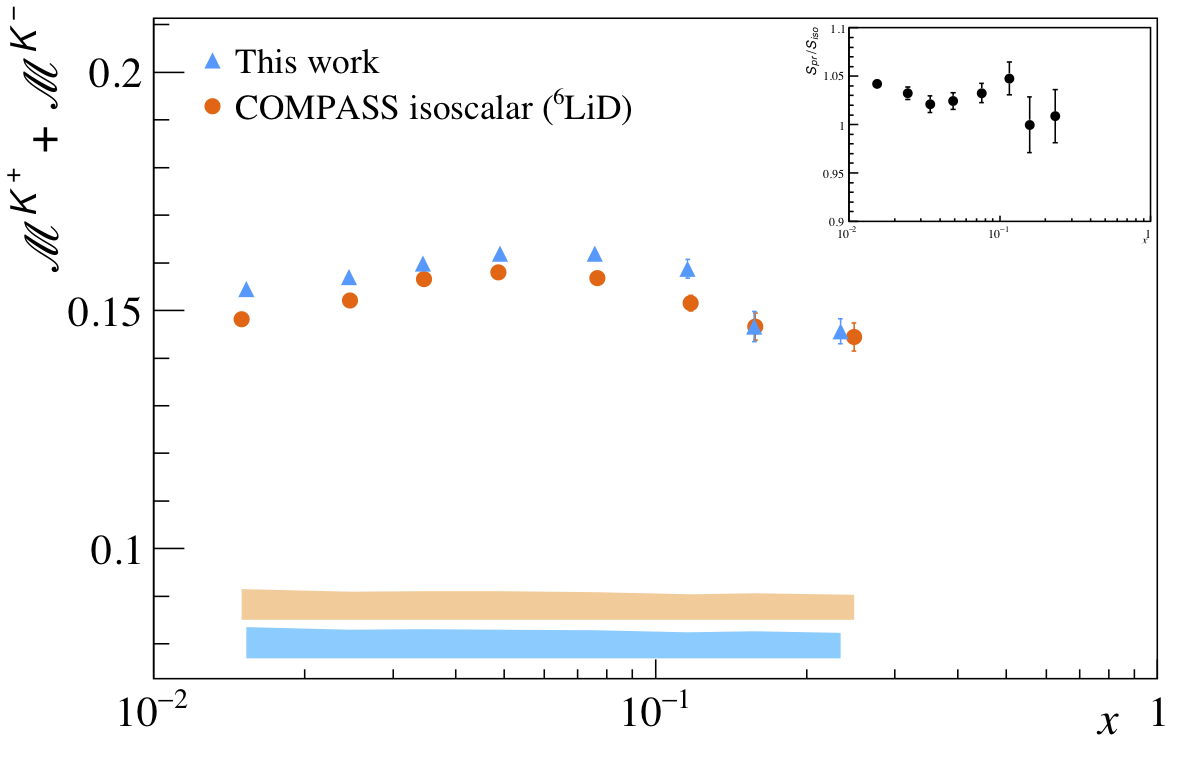
\includegraphics[scale=0.5]{./gfx/Ks_noH.png}
  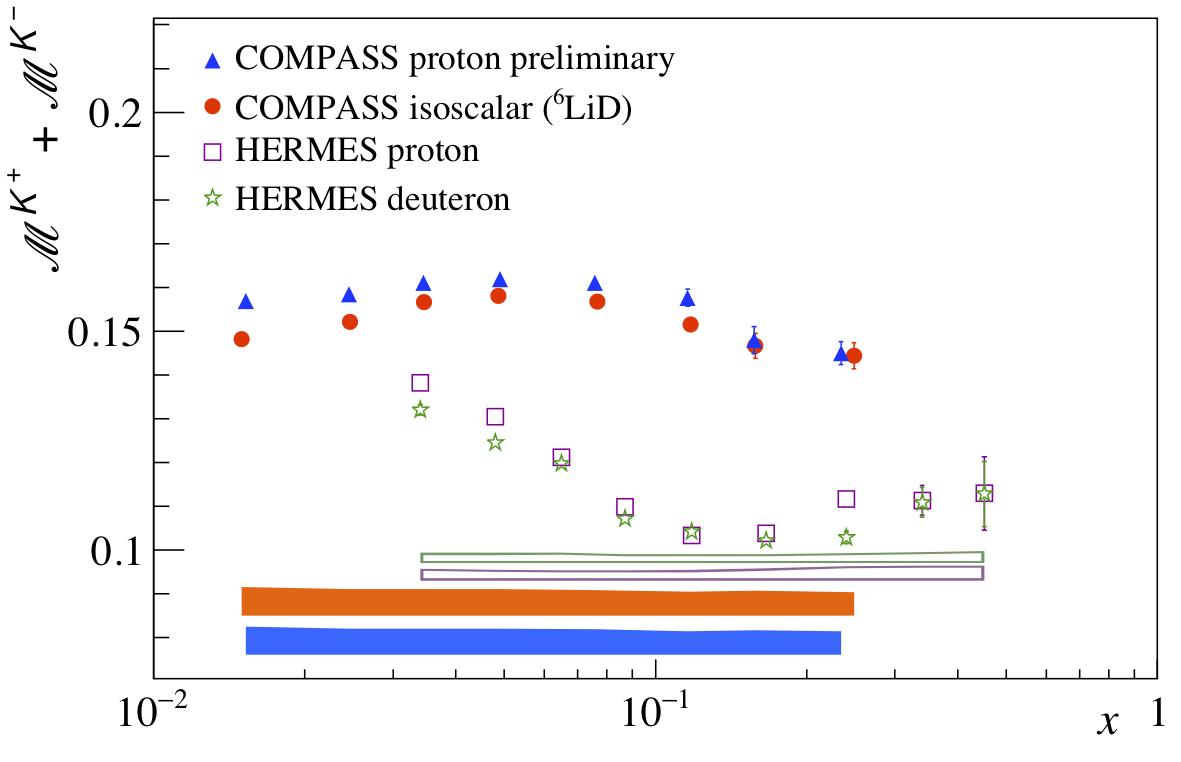
\includegraphics[scale=0.5]{./gfx/Ks.png}
  \caption{Sum of $\mathscr{M}^{K^+}+\mathscr{M}^{K^-}$ from COMPASS for a proton target (blue closed points) and an isoscalar target (orange closed points) and from HERMES for a proton target (violet open points) and a deuteron target (green open points).}
  \label{pic:ksum}
\end{figure}

The sum of charged kaon multiplicity $\mathscr{M}^{K^+}+\mathscr{M}^{K^-}$ for a proton target should be slightly ($\sim$5-10\%) above COMPASS results on isoscalar target. For the isoscalar results for kaons, contrary to hadrons and pions, an additive correction of $5\%$ was applied to the published results to take into account radiative correction as estimated at the time. The discrepancy with HERMES results, already seen in the isoscalar case, remains. As for the pions, the discrepancy between COMPASS results and HERMES results, both for a proton and deuteron targets, has to be noted. They lie well below the COMPASS points and exhibit a different $x$ behaviour. Towards low $x$, COMPASS data show a flat behaviour, unlike the rise that is suggested by the HERMES data. The explanations made for the pions concerning the discrepancies with HERMES are also valid for the kaons.

\subsection{Sum of proton/antiproton multiplicities}

In Fig. \ref{pic:psum}, the $\mathscr{M}^{p}+\mathscr{M}^{\bar{p}}$ from COMPASS is depicted for a proton target (blue points). This is the first time that this quantity is measured.

\begin{figure}[!h]
  \centering
	\includegraphics[scale=0.5]{./gfx/ps.png}
	\caption{Sum of $\mathscr{M}^{p}+\mathscr{M}^{\overline{p}}$ for COMPASS on proton target (blue closed points).}
	\label{pic:psum}
\end{figure}

\newpage

\section{Summary}

The final unidentified hadron ($h^{\pm}$), pion ($\pi^{\pm}$), kaon ($K^{\pm}$) and proton/antiproton ($p/\bar{p}$) multiplicities extracted from 2016 COMPASS data of muon deep inelastic scattering on a pure proton (lH$_2$) target were presented as a function of $z$ and in bins of $x$ and $y$. Averaging these results over $y$, two dimensional projection are obtained. The subsequent integration over $z$ allows the comparison of the sum and ration of charged hadron multiplicities with COMPASS results for an isoscalar target \cite{COMPASS2006Pi,COMPASS2006K} and with the HERMES experiment results \cite{HERMESMult}. For the ratio, every results are in agreement with the expectations relative to the COMPASS results for an isoscalar target. The discrepancy that was already observed for the kaon ratio between COMPASS and HERMES for a deuteron/isoscalar target is also present for a proton target. For the sum, the results for hadrons and pions differs from the expectations relative to the COMPASS results for an isoscalar target in the high $x$ region. Overall, all the results for a proton target for the sum seem to suffer from a drop at high $x$, particularly visible on hadrons and pions, which should be flat. The kaons seem to be less harmed by this issue. The cause of this drop is still under investigation and might probably be caused by a bad tuning of some hadron variables. Nevertheless, comparing with HERMES results, a great discrepancy is observed at low $x$ in the pion case while in the kaon case, a major discrepancy is observed for all $x$. The proton results should interest the community as there is at the moment no major data set released for them.
